\documentclass[12pt]{ociamthesis}

\listfiles

%load any additional packages
\usepackage{amssymb}
\usepackage{svg}
\usepackage[nottoc,numbib]{tocbibind}
\usepackage{listings}
\usepackage{graphicx}
\usepackage{nameref}
\usepackage{titlesec}
\usepackage{csquotes}
\usepackage[english]{babel}
\usepackage[T1]{fontenc}
\usepackage[sorting=nyt,style=apa,backend=biber]{biblatex}
\DeclareLanguageMapping{english}{english-apa}
\usepackage[hidelinks]{hyperref}

\bibliography{refs}        %use a bibtex bibliography file refs.bib

\graphicspath{{images//}}

\titleformat{\chapter}
	{\normalfont\LARGE\bfseries\color{black}}{\thechapter.}{.1em}{}

\titleformat{\paragraph}
{\normalfont\normalsize\bfseries}{\theparagraph}{1em}{}
\titlespacing*{\paragraph}
{0pt}{3.25ex plus 1ex minus .2ex}{1.5ex plus .2ex}

\renewcommand{\theparagraph}{\roman{paragraph}}

\title{Real-time Visual Effects with GPU Ray-tracing of Volume Data}

\author{Caitlin Wilks\\cat@wilks.so}

\college{School of Computing \& Mathematics}

%\renewcommand{\submittedtext}{change the default text here if needed}
\degree{BSc (Hons) Computer Games Programming}    	%the degree
\degreedate{in the years 2013-2014}         							%the degree date

%end the preamble and start the document
\begin{document}

%this baselineskip gives sufficient line spacing for an examiner to easily
%markup the thesis with comments
\baselineskip=18pt plus1pt

\setcounter{secnumdepth}{4}
\setcounter{tocdepth}{2}

\maketitle                  % create a title page from the preamble info
\begin{abstract}
Welcome to abstract, home of the abstract, can I take your order?
\end{abstract} % include the abstract

\begin{romanpages}          % start roman page numbering
\tableofcontents            % generate and include a table of contents
\newpage
\listoffigures              % generate and include a list of figures
\end{romanpages}            % end roman page numbering

% Include chapters
\section{Introduction}
\section{Literature Review}
\chapter{Methodology}
\label{methodology}

\section{Ray tracing}
Our ray tracer uses the GPU-optimised parametric octree traversal algorithm presented by \cite{laine10efficientsvos}. This algorithm is extremely efficient for traversing along rays through a sparse octree as it hierarchically avoids empty space, finding the first intersection of the ray extremely fast.

\begin{figure}
\centering
	\centering
	\subfloat[Intersection of the root with the ray]{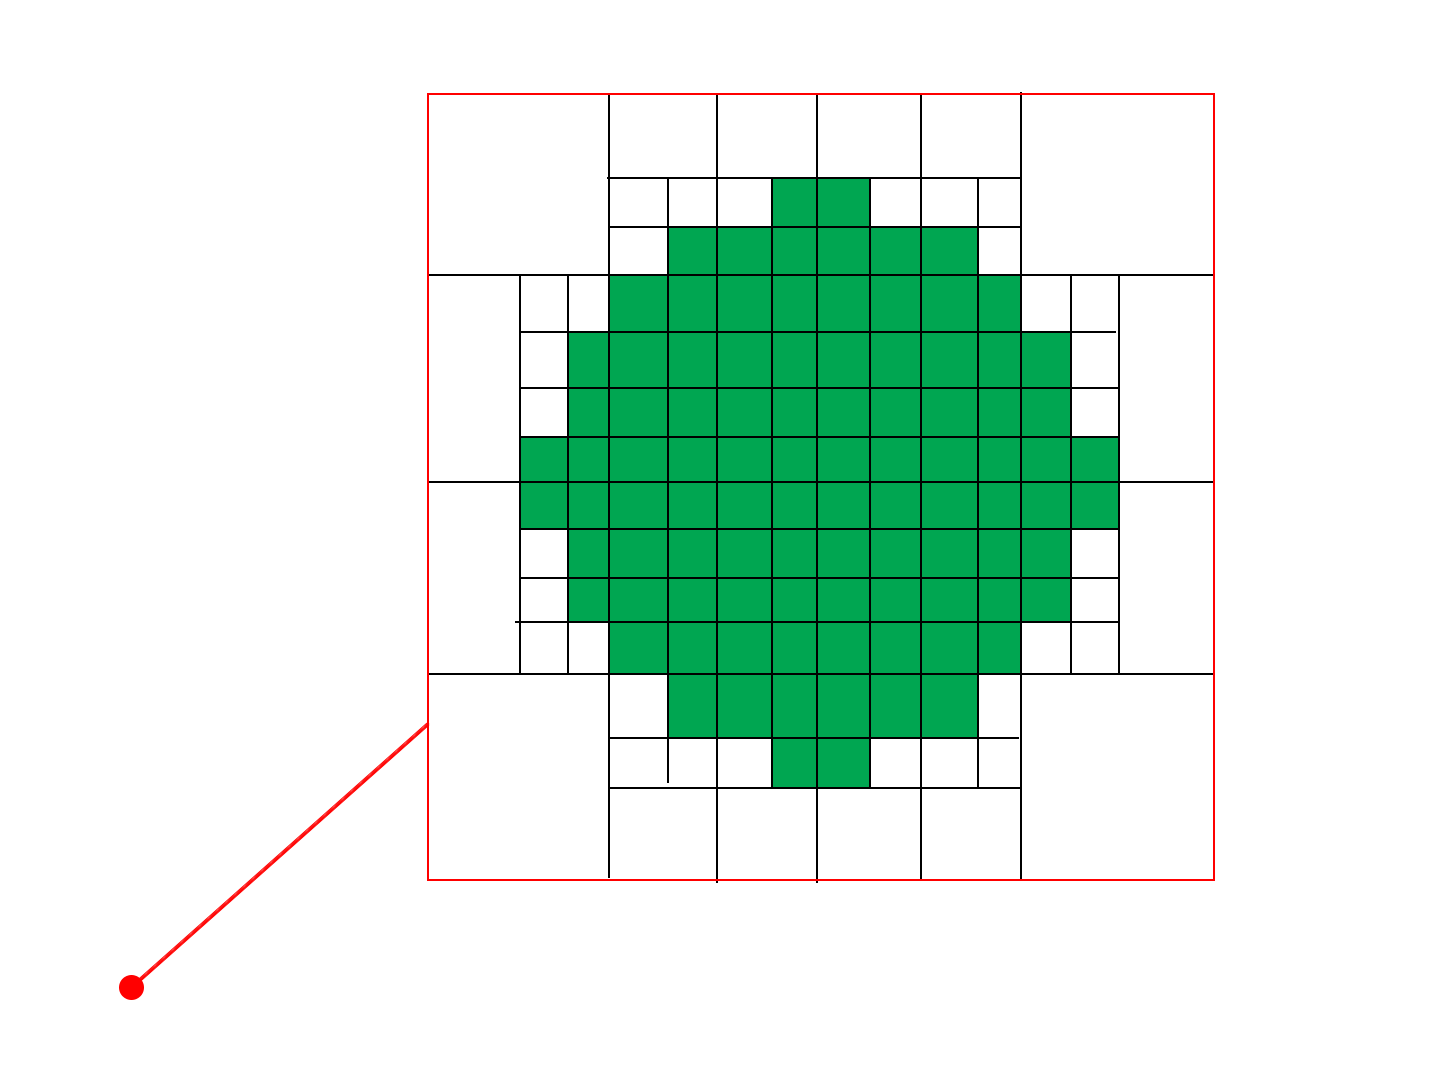
\includegraphics[width=3in]{initial_intersection.png}}
	~
	\subfloat[Initial child selection]{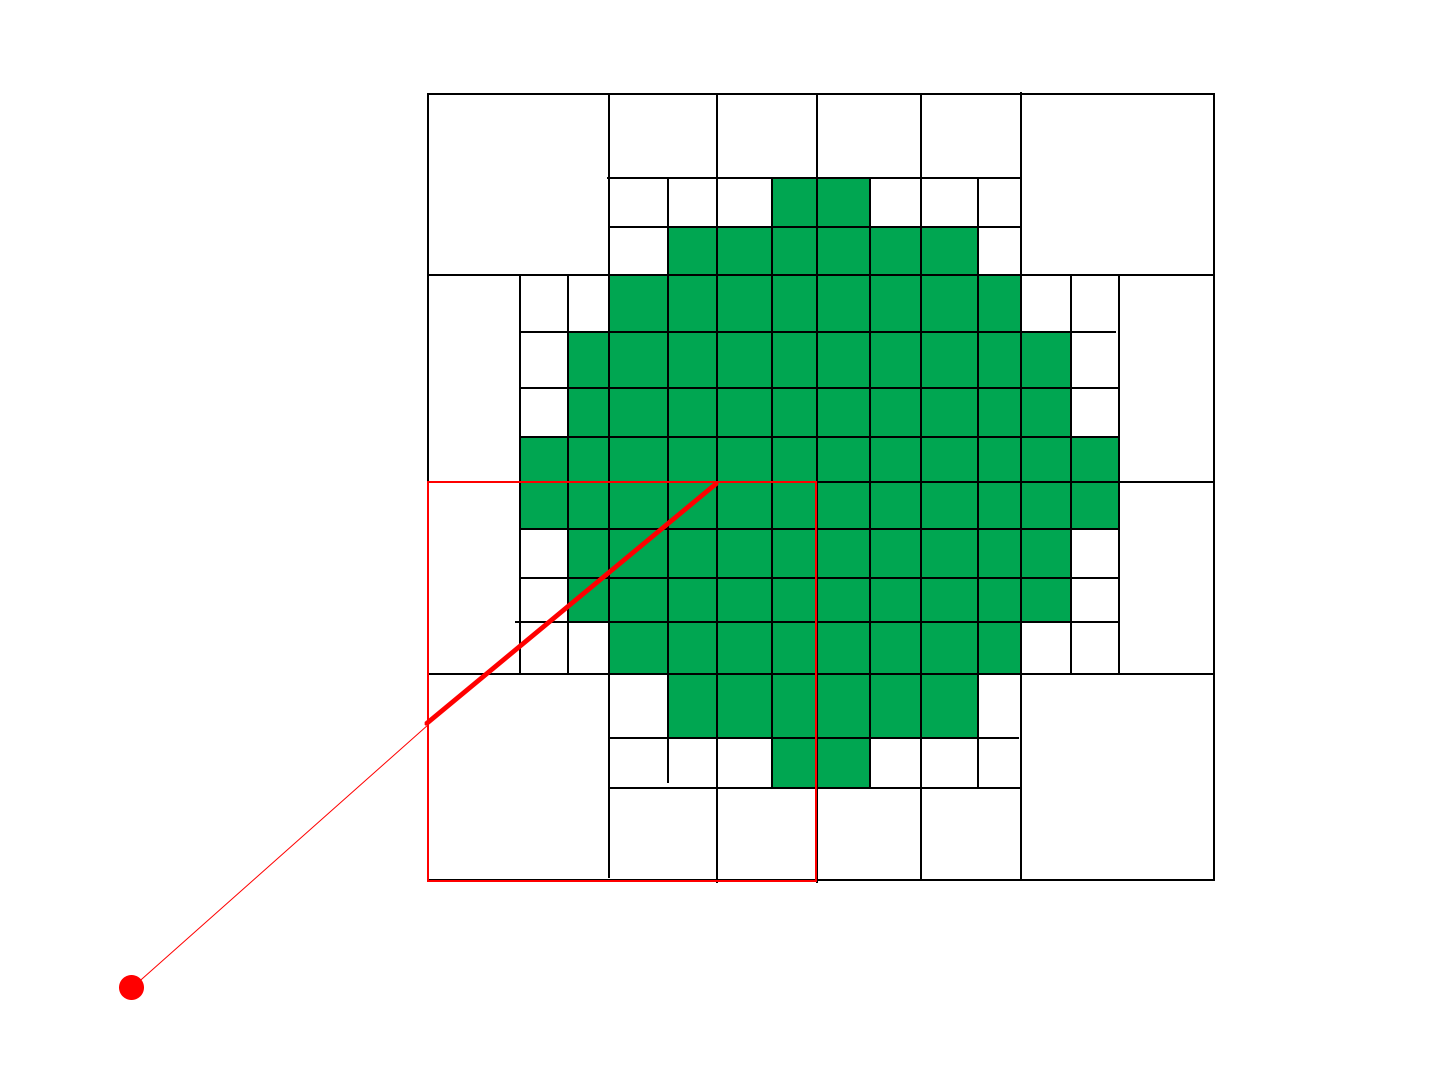
\includegraphics[width=3in]{initial_intersection_child.png}}

	\caption{Initial intersection test}
	\label{fig:root_intersect}
\end{figure}

Pseudo-code for the ray casting algorithm is given in algorithm \ref{alg:raycast}. Our data is stored in a regular octree structure, meaning that each node of the tree is divided into 8 identically sized octants. The algorithm then begins by determining the intersection of the root node with the ray, as well as determining the first entered child octant. This is shown in figure \ref{fig:root_intersect}. The main loop then begins.

\begin{algorithm}
\caption{Ray cast algorithm pseudo-code \parencite{laine10efficientsvos}}
\label{alg:raycast}
\begin{algorithmic}[1]
\Procedure{Raycast}{$root, ray$}
	\State $current\_voxel \gets intersect(root,~ray)$			\Comment{Intersection with root}
	\While{$not~terminated$} \Comment{Traverse}
		\If{$current\_voxel~exists$}
			\If{$voxel~smaller~than~pixel$} 					\Comment{Exit conditions}
				\State $\textbf{return}~current\_voxel$
			\ElsIf{$voxel~is~a~leaf$}
				\State $\textbf{return}~current\_voxel$
			\Else
				\State $current\_voxel \gets push(currrent\_voxel, ray)$		\Comment{Descend into child}
			\EndIf
		\EndIf

		\State $current\_voxel \gets advance(current\_voxel, ray)$			\Comment{Advance into next sibling}

		\If{$advance~direction~disagrees~with~ray~direction$}
			\State $current\_voxel \gets pop(current\_voxel, old\_voxel)$			\Comment{Pop last common parent}
		\EndIf
	\EndWhile
\EndProcedure
\end{algorithmic}
\end{algorithm}

The algorithm then checks that the current voxel exists. If the current voxel exists, the exit conditions are checked: the projection of the current voxel is smaller than the pixel on-screen, and whether the voxel is a leaf node, in which case there are no more subdivisions below it. If either of these conditions are met, the algorithm terminates, returning the current voxel. Otherwise, the algorithm executes push, advancing the traversal to the first entered child voxel.

\begin{figure}
\centering
	\centering
	\subfloat[The current voxel prior to push]{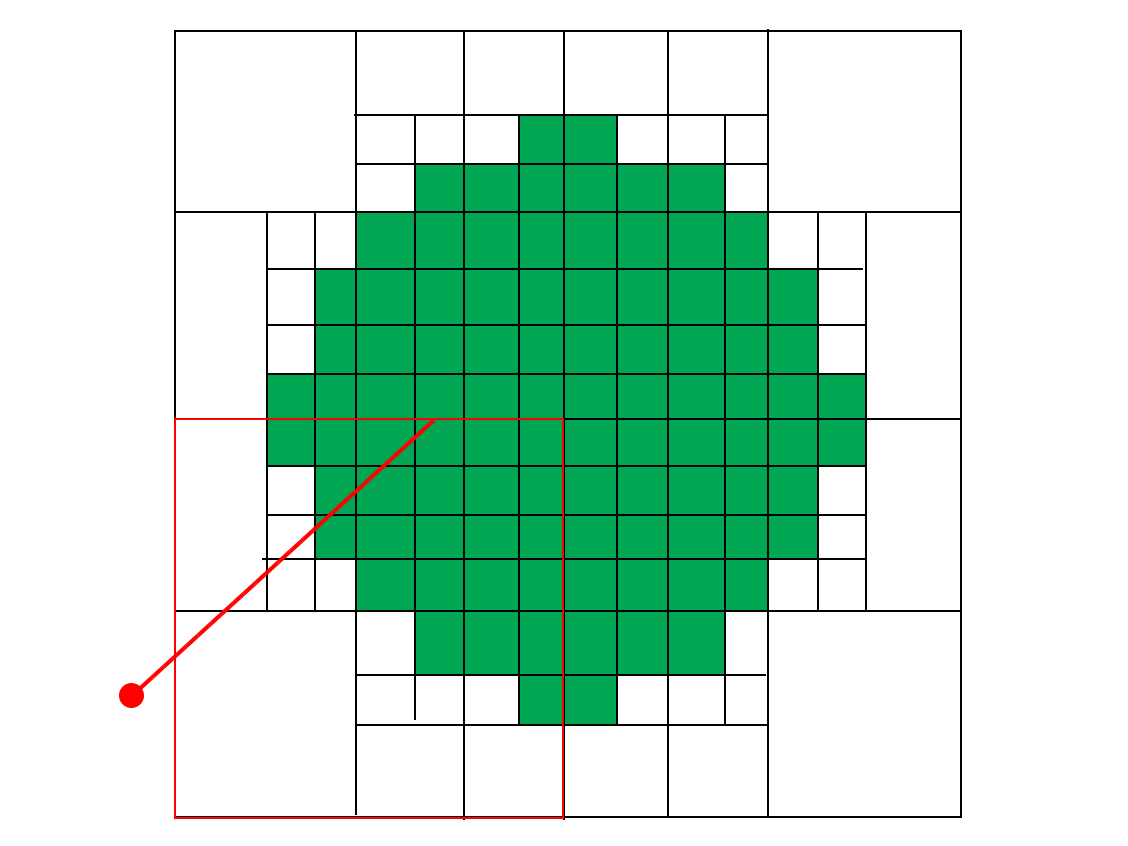
\includegraphics[width=3in]{push_initial.png}}
	~
	\subfloat[The current voxel after push]{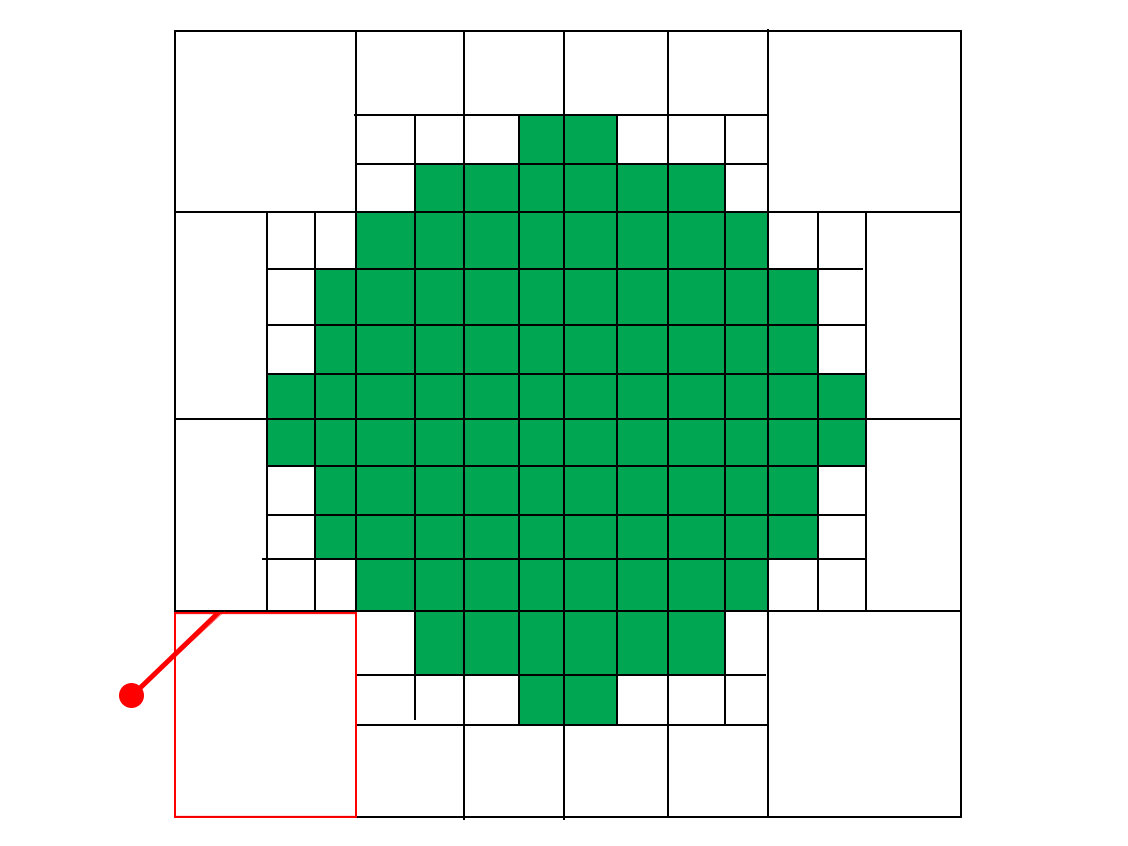
\includegraphics[width=3in]{push_post.png}}

	\caption{The push operation, 2D case}
	\label{fig:ray_push}
\end{figure}

If the current voxel does not exist, the algorithm advances the traversal to the next voxel intersected by the ray on the current level. The direction of advancement is then checked against the ray direction to ensure the advance was valid. If the direction of advance does not coincide with the direction of the ray, in which case one of the parent nodes of the current voxel differs from one of the parent nodes of the previous voxel, pop is used to return to the last common parent of the two voxels and determine the next child intersection along the ray, after which time traversal continues. The push, advance, and pop operations are described fully by \cite{laine10efficientsvos}.

\begin{figure}
\centering
	\subfloat[The current voxel prior to advance]{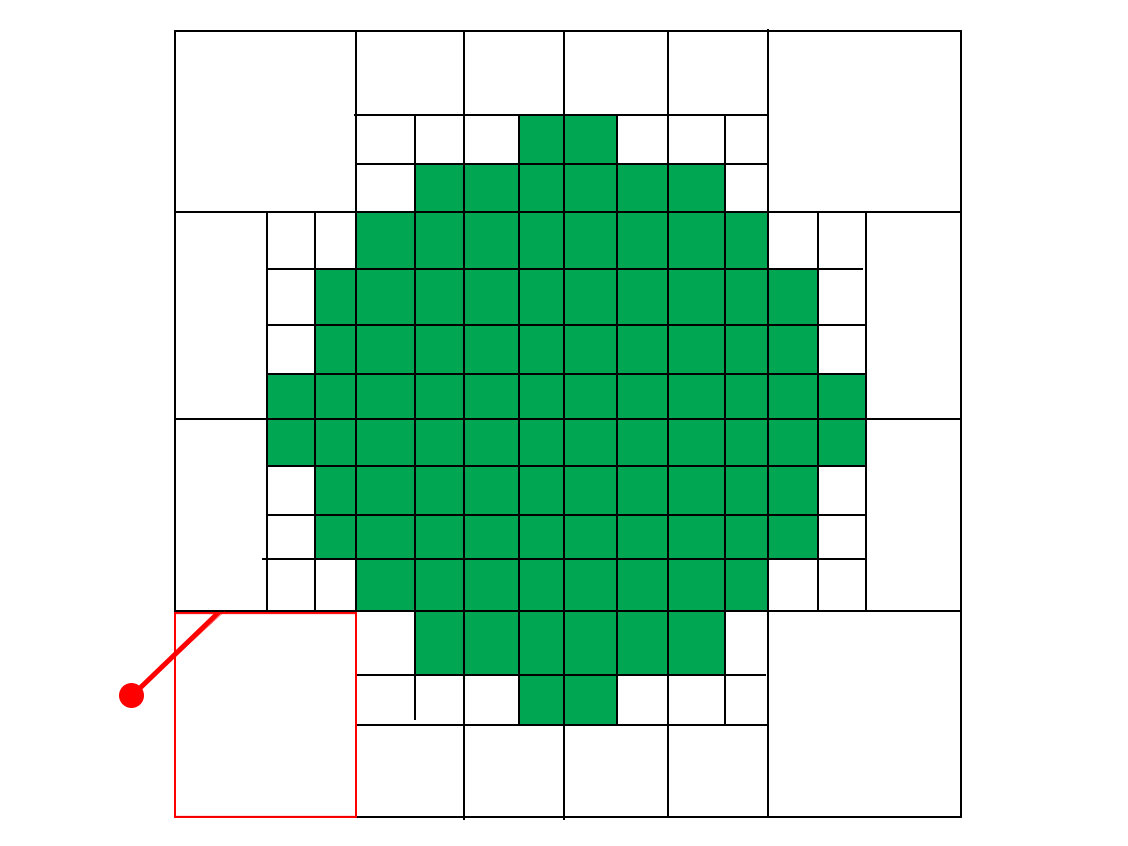
\includegraphics[width=3in]{push_post.png}}
	~
	\subfloat[The current voxel after advance]{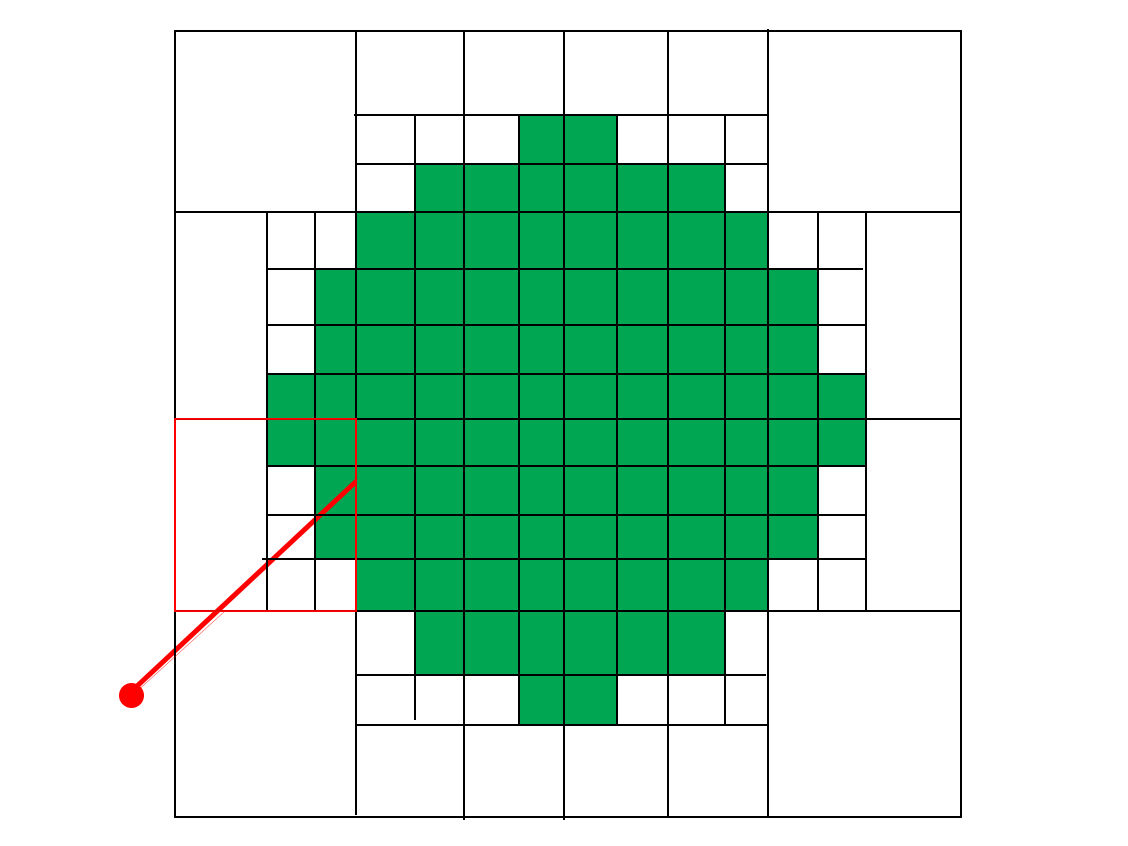
\includegraphics[width=3in]{advance_post.png}}

	\caption{The advance operation, 2D case}
	\label{fig:ray_advance}
\end{figure}

As empty space is quickly advanced over, preventing unnecessary traversal deeper into the tree, and voxels are never revisited, this algorithm quickly determines whether a ray intersects with a volume stored within an octree. This efficient traversal allows us to cast rays against a volume to produce a real-time ray traced image.

\begin{figure}
\centering
	\subfloat[The initially intersected voxel]{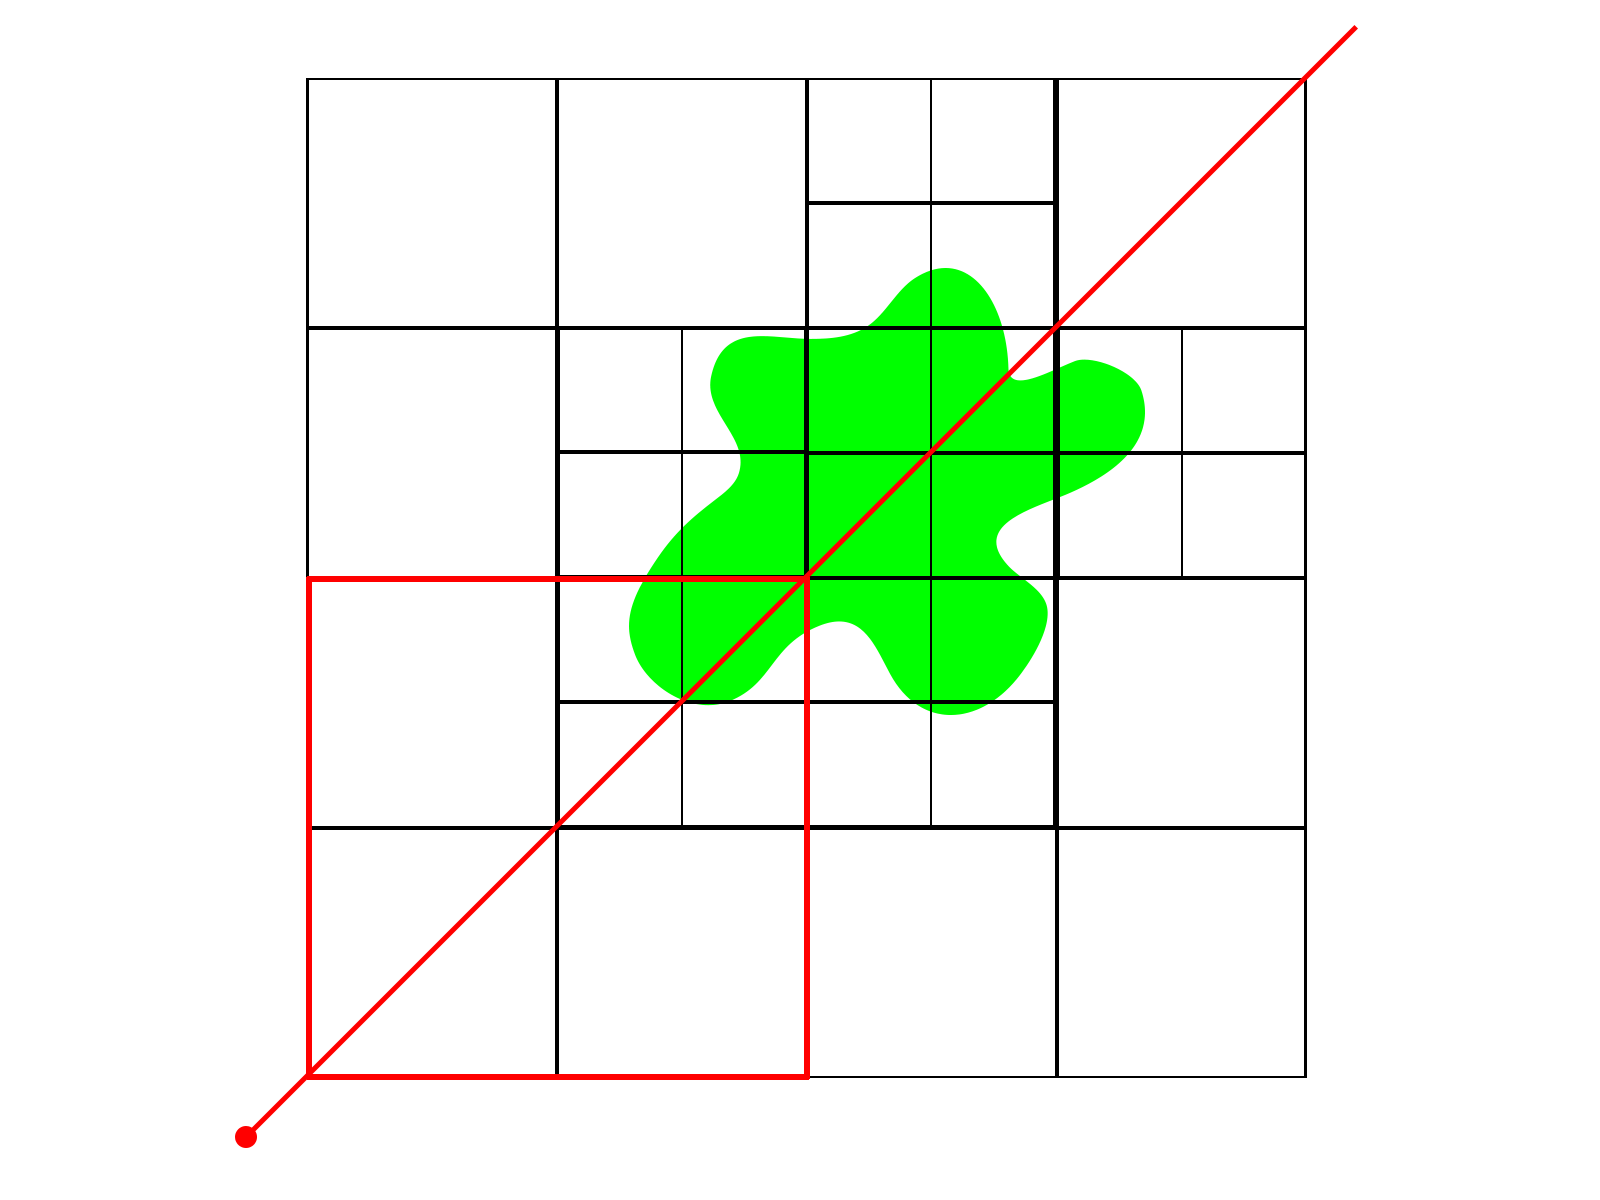
\includegraphics[width=3in]{emptyspace_1.png}}
	~
	\subfloat[Push]{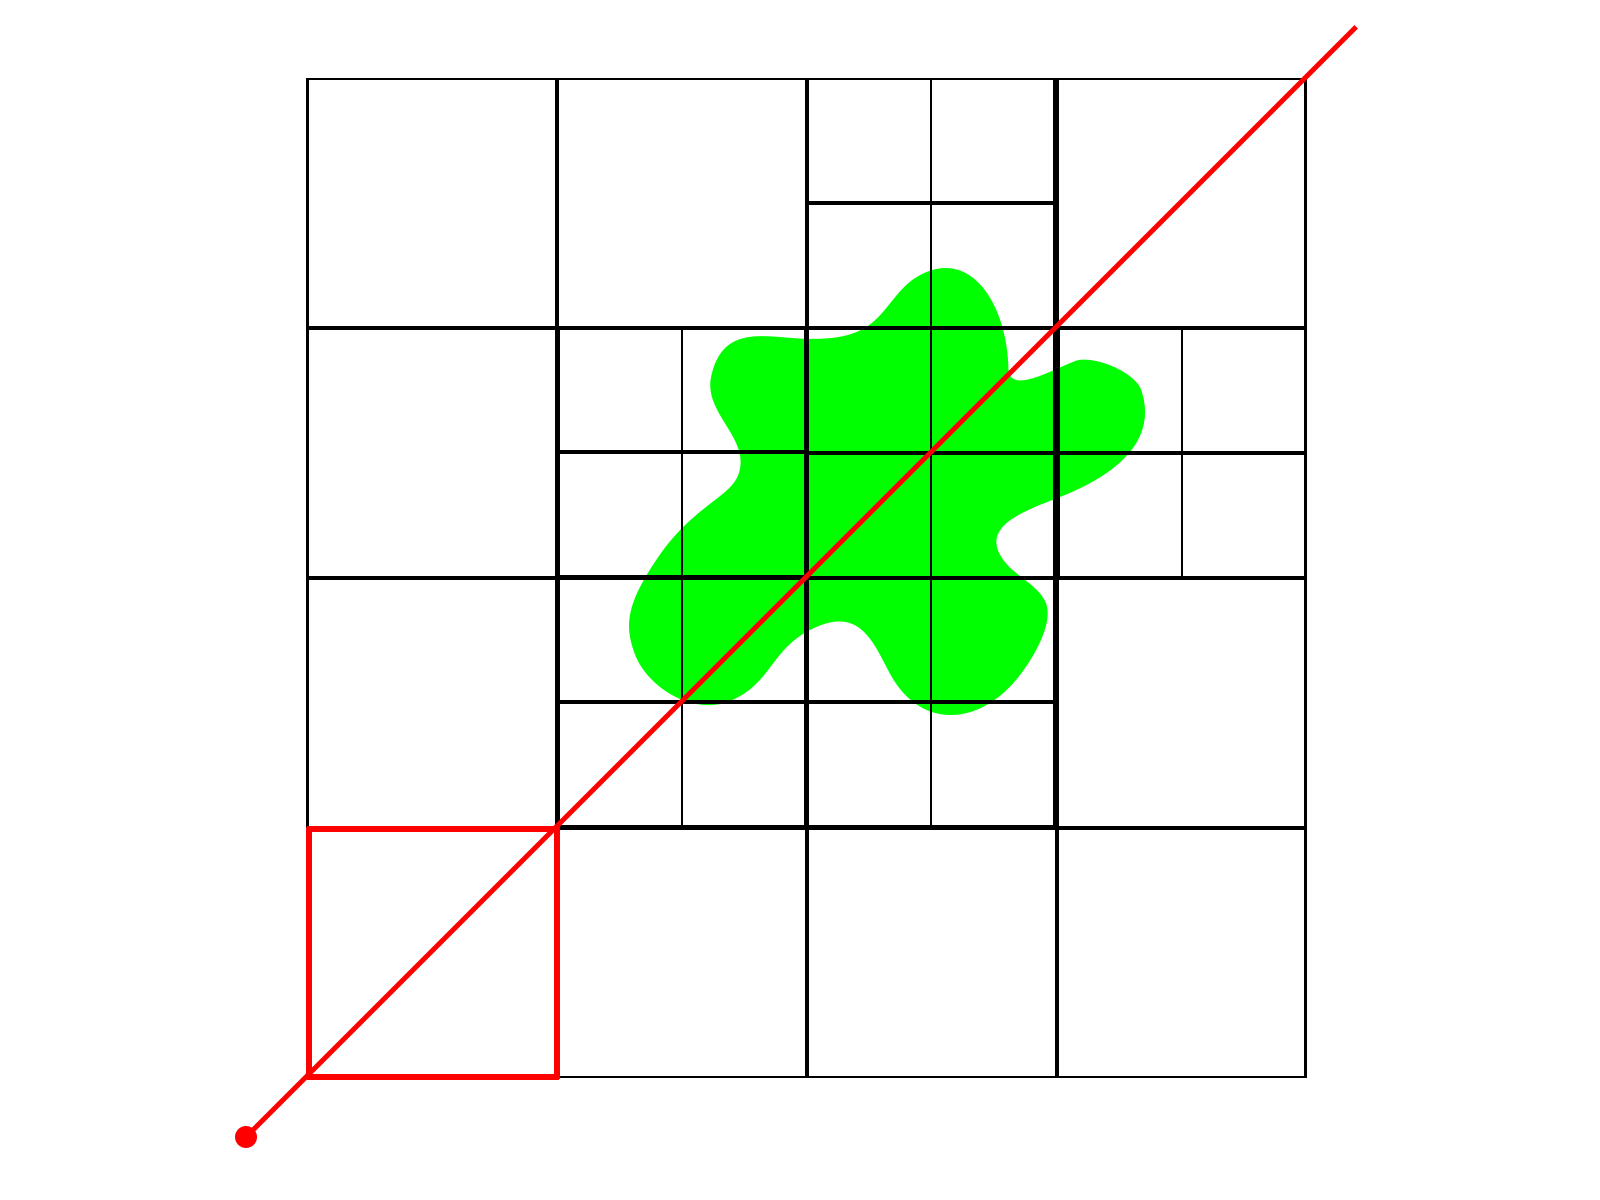
\includegraphics[width=3in]{emptyspace_2.png}}
	\\
	\subfloat[Advance]{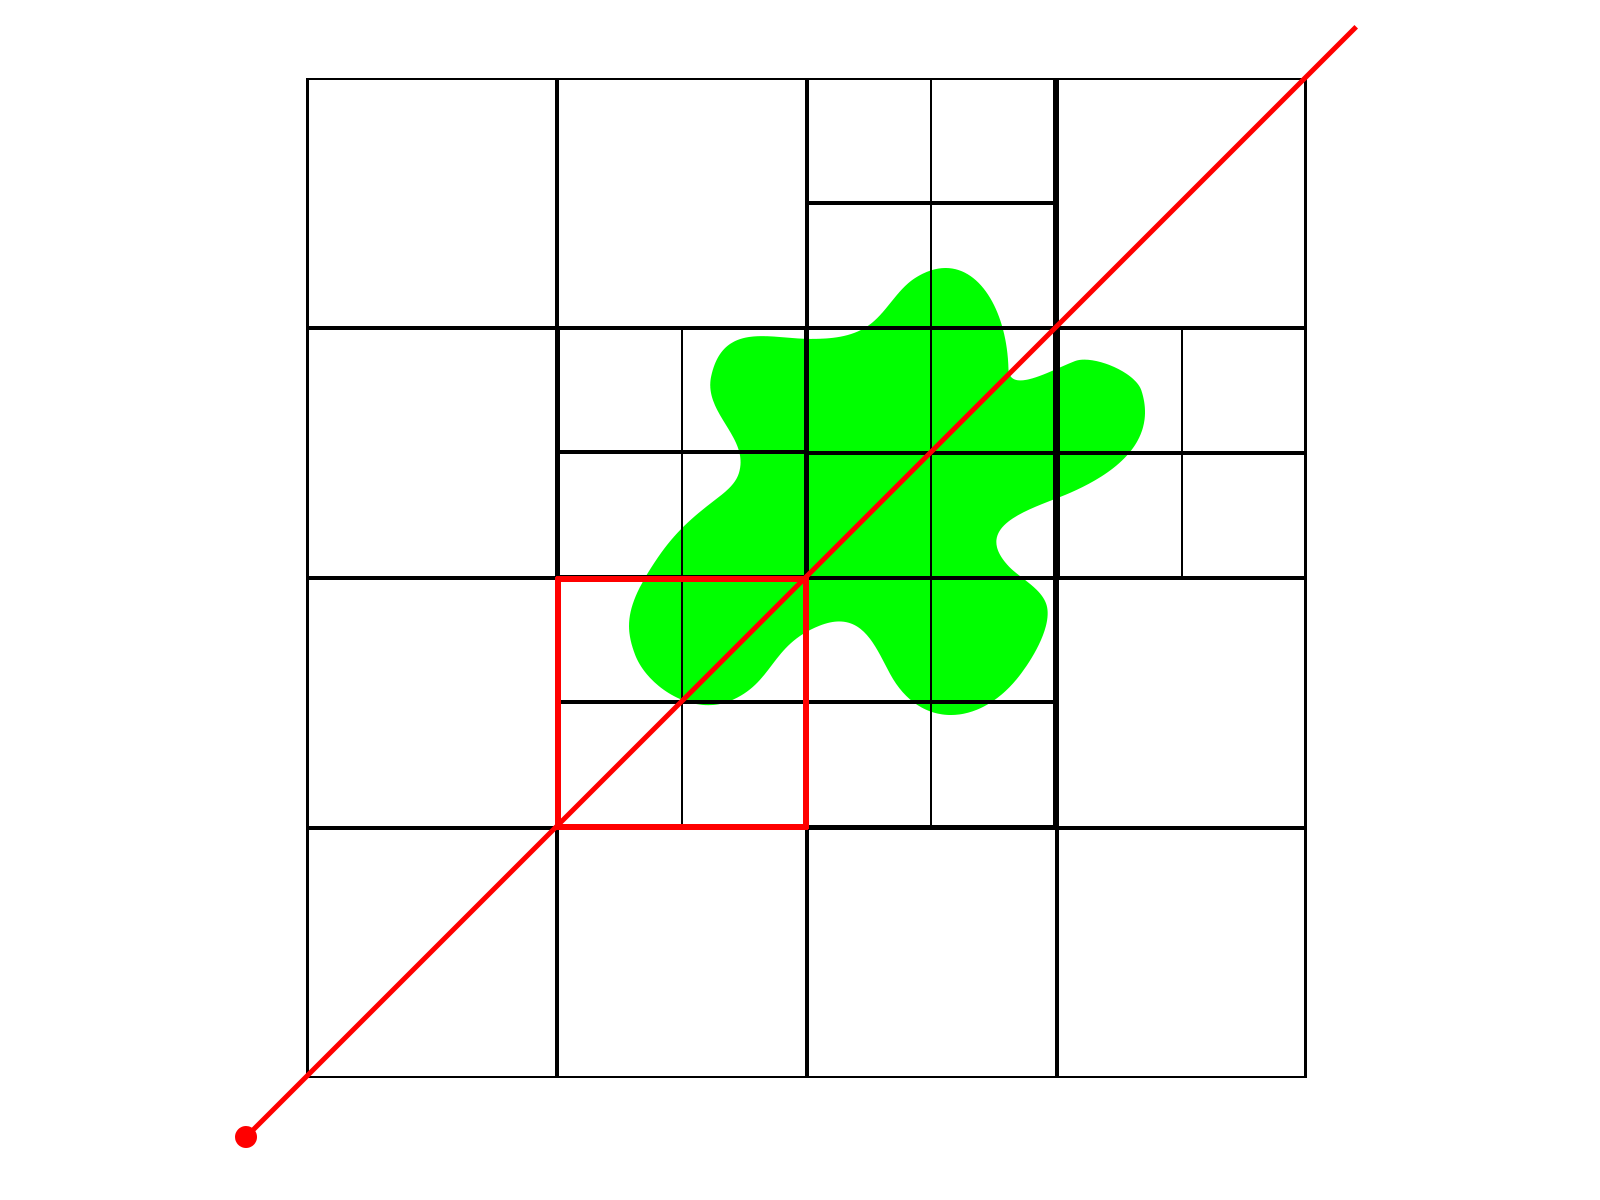
\includegraphics[width=3in]{emptyspace_3.png}}
	~
	\subfloat[Push]{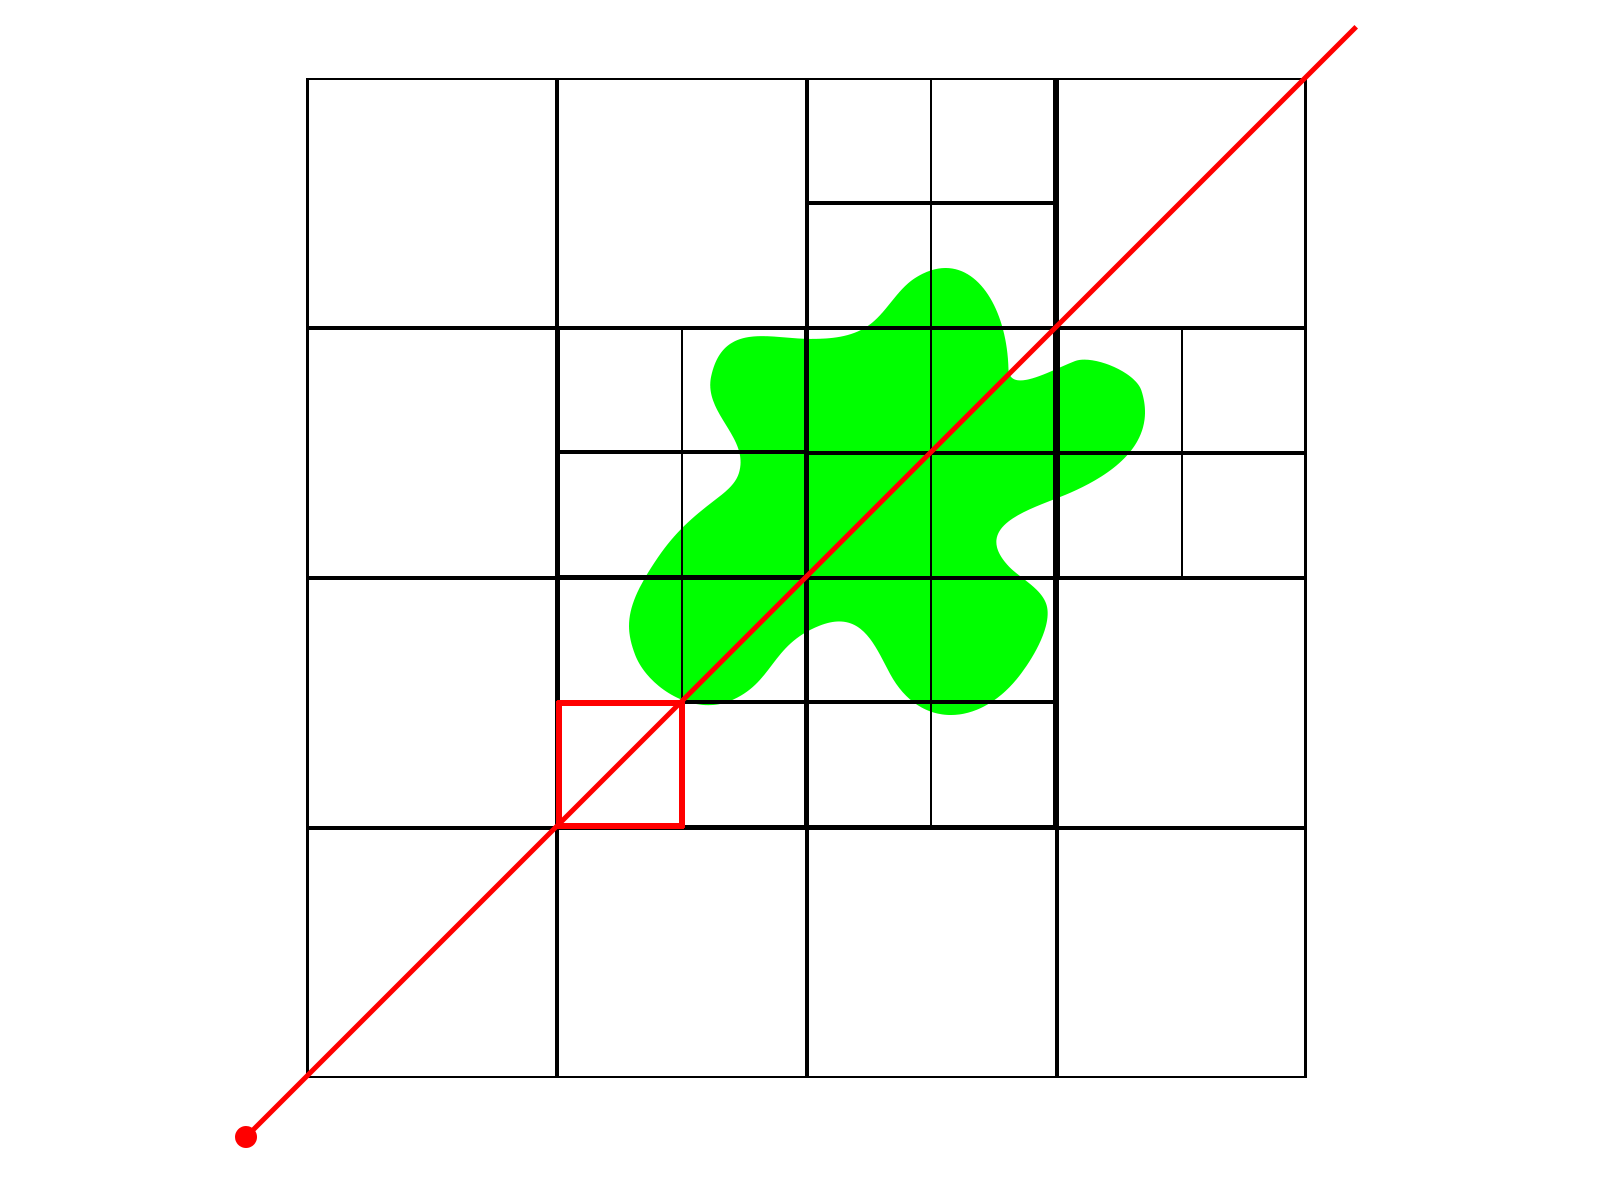
\includegraphics[width=3in]{emptyspace_4.png}}
	\\
	\subfloat[Advance, the first intersected voxel is found]{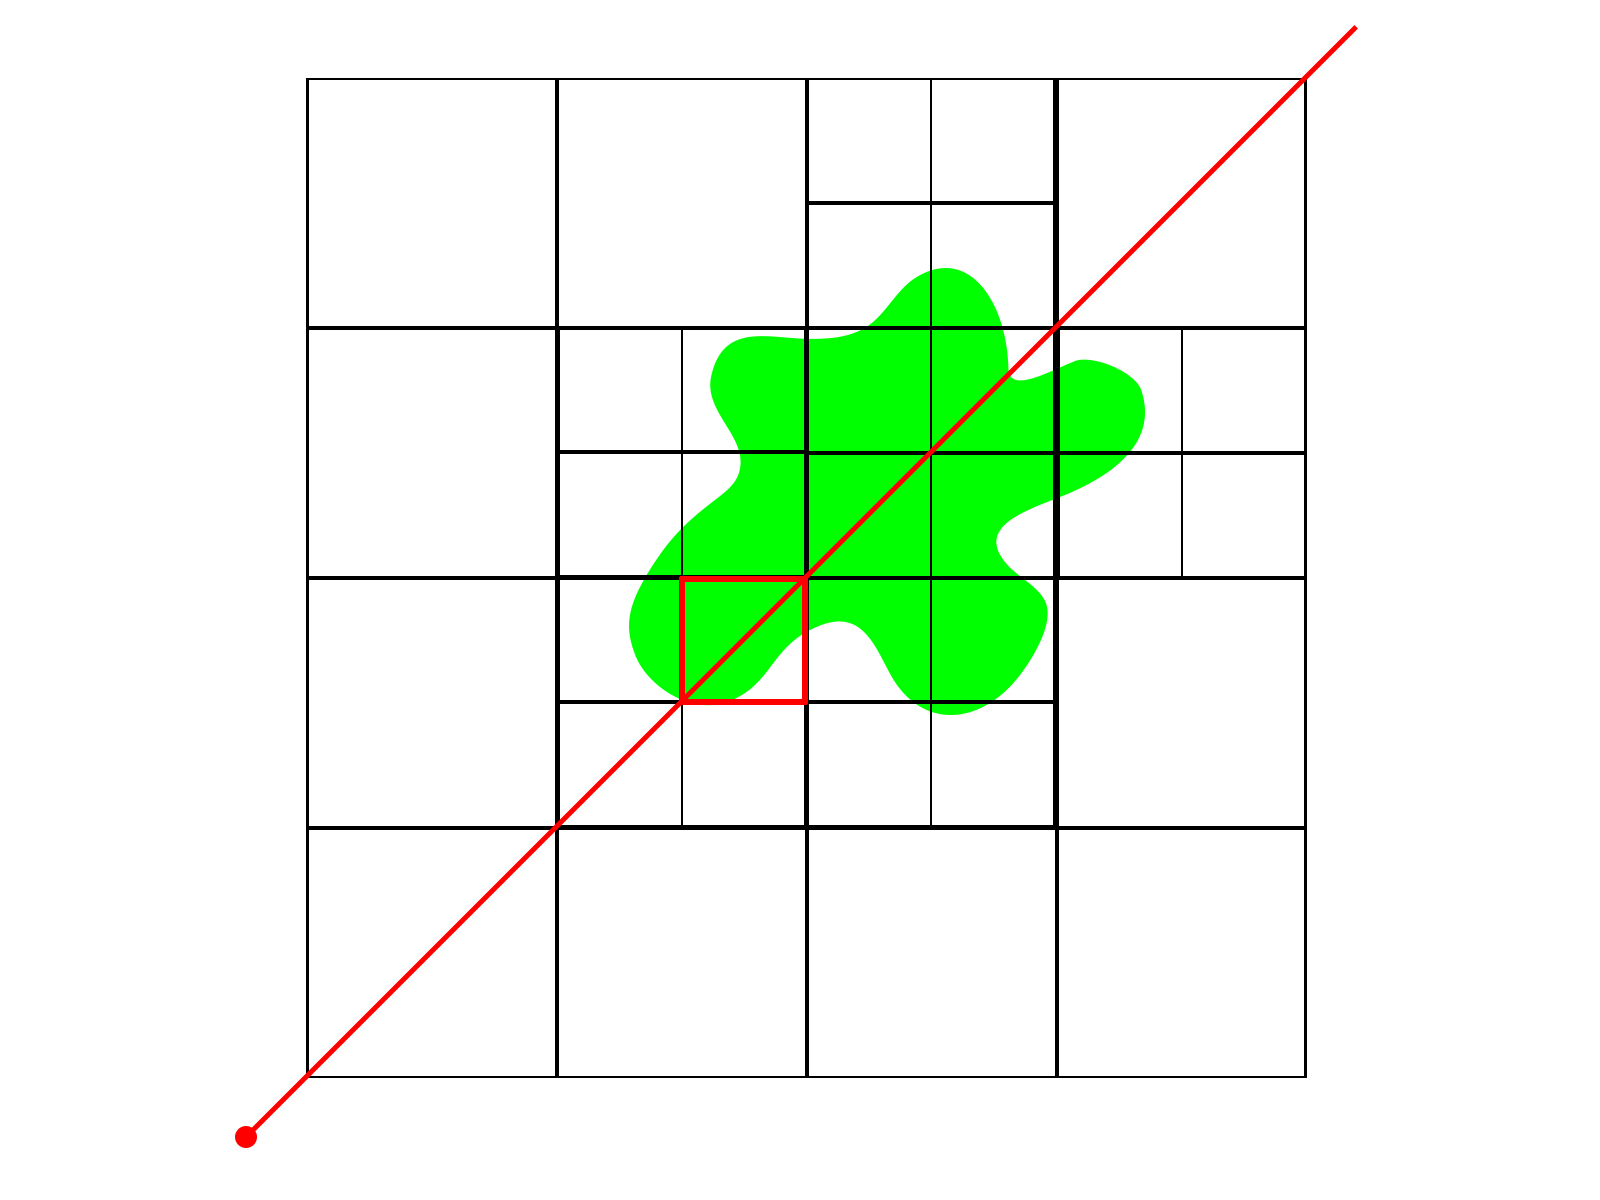
\includegraphics[width=5in]{emptyspace_5.png}}

	\caption{How empty space is avoided, 2D case}
	\label{fig:empty-space}
\end{figure}

\subsection{Storage}
Our data structure uses the same basic storage mechanisms as \cite{laine10efficientsvos}. The tree structure is stored separately from the related shading data, as the majority of processing time is spent in traversal. The extra time it takes to look up shading attributes for shading is therefore traded for a more compact traversal structure. A pointer to a lookup table pointing to attributes for the whole volume is stored at 8 kilobyte boundaries within the tree data.

The tree structure encodes each non-leaf node as a child descriptor, containing a pointer to the children of the current node, an 8-bit mask detailing which of the current node's children exists, and another 8-bit mask which determines which of the node's children are non-leaves (in other words, which children have their own child descriptors stored at the child pointer.)

The child descriptors for the children of a node are then stored together in a block, referenced by this child pointer. The non-leaf mask can then be used to access a particular child using an index from 0 to 7 using a 256 bit lookup table which relates the non-leaf mask of a parent voxel to the index of the desired child:

\[
	child\_offset = lookup(non\_leaf\_mask << child\_index)
\]

The lookup table contains values from 0 to 7, containing the offset of the desired child given a particular non-leaf mask. This lookup table and the relevant implementation is shown in appendix \ref{app:lookup-table}.

\subsubsection{Voxel attributes}
The attributes stored for each voxel are the main way in which our storage scheme varies from that used in \cite{laine10efficientsvos}. In \cite{laine10efficientsvos}, only a colour and a normal, representing the volume after ambient occlusion is pre-calculated, are required for shading. For our purposes, additional attributes are required per-voxel, such as index of refraction and reflectance.

Attributes are stored after the traversal information, along with a lookup table that points to blocks of attributes, grouped by parent voxel. The index in the lookup table can be obtained by considering the offset of the parent's child descriptor from the start of the data, as so:

\[
	lookup\_index = \frac{parent\_desc\_addr - start\_addr}{child\_desc\_size}
\]

The child descriptor size is a constant, referring to the size in bytes of each child descriptor.

This index is then used to retrieve the block of attributes containing the current voxel's attributes, and then the $child\_offset$ obtained above is used to obtain the attributes for the current voxel:

\[
	voxel\_attributes = lookup\_table[lookup\_index] + child\_offset
\]

The resulting pointer points to a structure containing the packed attributes required to shade the current voxel. For our renderer, that includes colour, normal, reflectance, and index of refraction, where the colour also contains an alpha channel which is used to determine transparency. The number of bits used to store each attribute is detailed below:\\

\begin{tabular}{|l|r|l|}
\hline

Attribute & Size in bits & Details \\
\hline

Colour	& 32 bits	& 8 bits for red, green, blue, and alpha components \\
		& 			& between 0.0 and 1.0 \\
\hline

Normal	& 32 bits	& Encoded as detailed in \cite{laine10efficientsvos}, \\
		&			& providing up to 14 bits of precision for smooth \\
		&			& normals \\
\hline

Reflectance & 16 bits & A floating point value between 0.0 and 1.0 \\
\hline

Index of refraction & 16 bits & A floating point value between 1.0 and 4.0 \\
\hline

\end{tabular} \\

The 16-bit floating point values for reflectance are stored as integers between $-2^{15}$ and $2^{15}$, as these are the minimum and maximum values that can be stored in a signed 16-bit integer. These values are scaled such that the minimum value (0.0 for reflectance and 1.0 for refraction) is encoded as $-2^{15}$, and the maximum value as $2^{15}$. Minimum and maximum values were chosen to maximise the precision of the packed values, although the values are packed as 16-bit integers purely for the reason that two 16-bit integers fit exactly into a 32-bit bit-field. If more attributes were added as needed, the sizes of these packed values could potentially be reduced as needed.

The minimum and maximum values for reflectance were chosen as values outside of this range are not physically sensible, as reflectance is defined as the fraction of received electromagnetic radiation (in this case, light) that is reflected by a surface. Values between 0 and 1 for refraction are also not physically sensible, although 4 was chosen as an arbitrary cut-off.

Floating point values are packed into integral bitfields using the following formula, where min and max are the minimum and maximum values to be considered, and bits is the number of bits allocated:

\[	range = max - min \]
\[	int\_max = 1 << (bits - 1) \]
\\
\[	packed\_value = floor((value - min) \cdot \frac{int\_max}{range}) \]

These values are then unpacked as needed. In some cases, this might not be necessary. For example, when checking for changes in index of refraction, the integral value can be used instead.

\section{Reflection rays}
\begin{figure}
\centering
	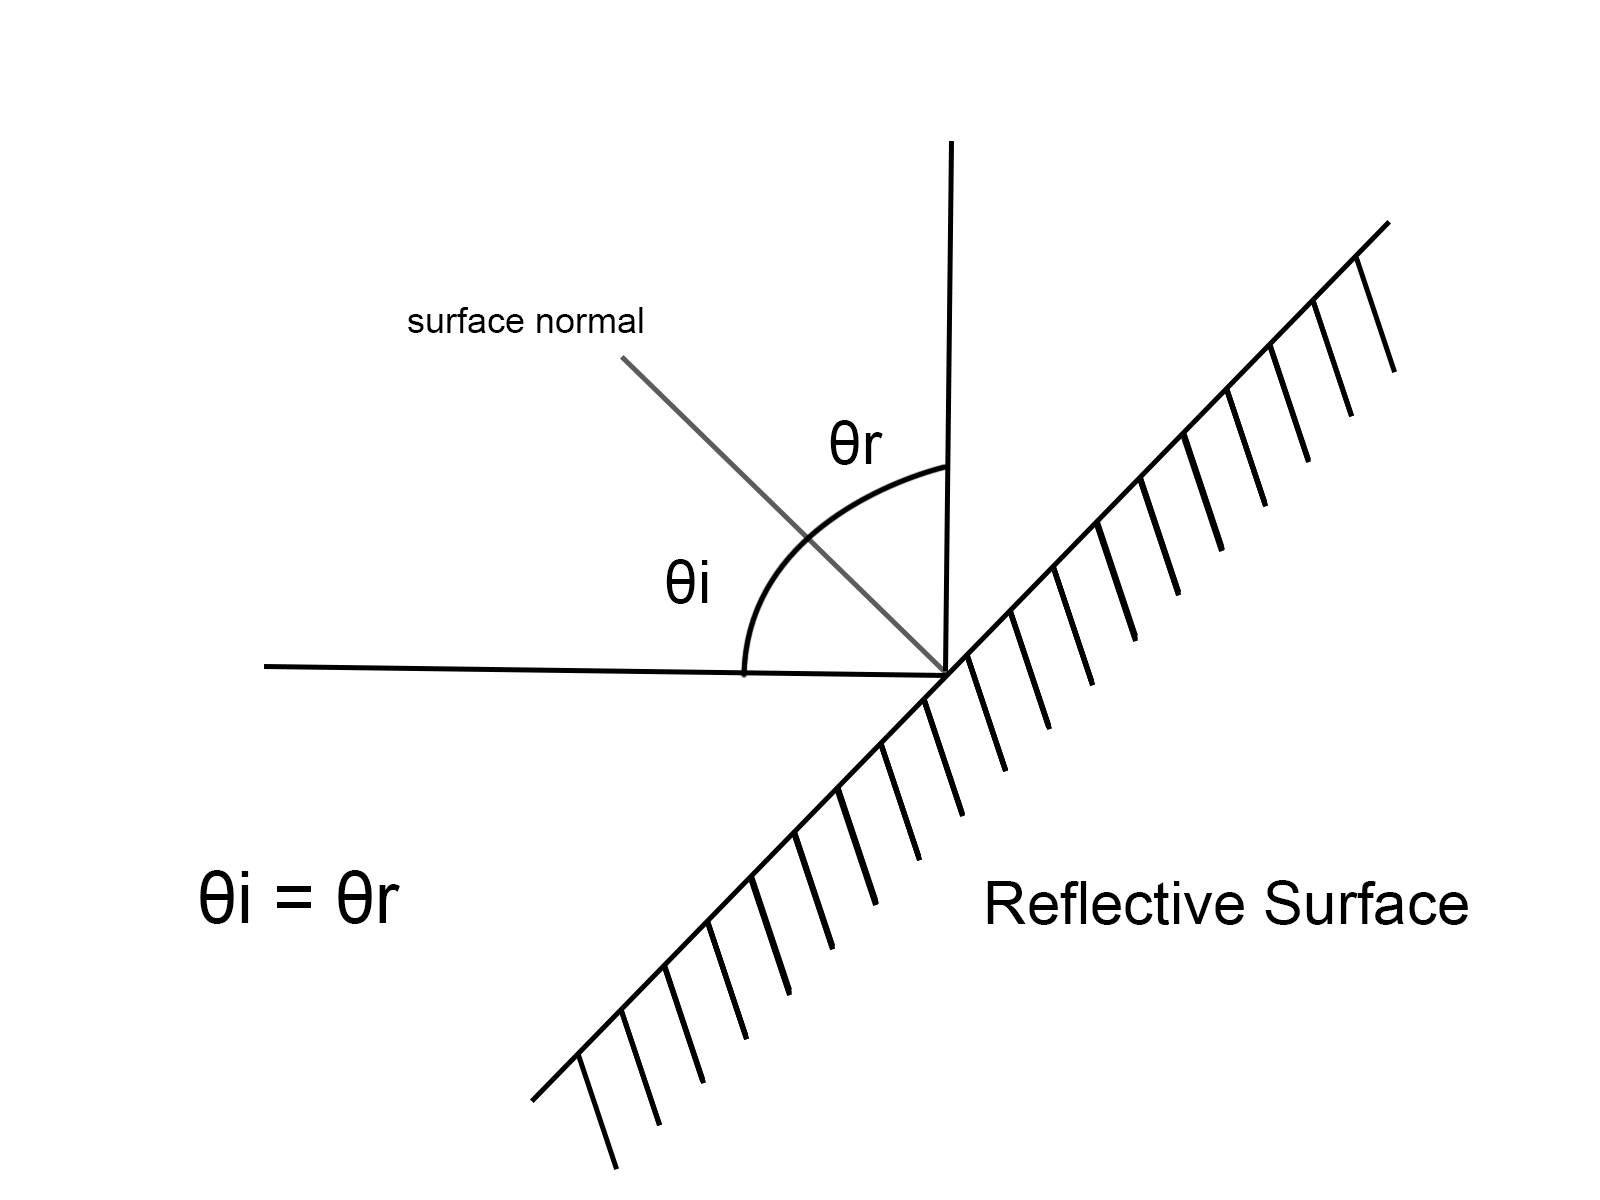
\includegraphics[width=14cm]{reflection.png}
	\caption{The relationship between the angle of incidence $\theta_i$ and the angle of reflection $\theta_r$}
	\label{fig:reflection}
\end{figure}

In order to determine the contribution of light reflected by the scene, a reflection ray must be cast in the angle of reflection in order to find any surfaces that may be reflecting light back. The law of reflection tells us that the angle of incidence, the angle between the normal of a surface and the ray hitting it, is equal to the angle of reflection \parencite{heath99history}. The GLSL (OpenGL Shader Language) specification gives a vector form of this equation using the dot product \parencite{glslspec}, where $I$ is the incident vector and $N$ is the normal of the surface:

\[
	reflection~direction = \vec{I} - 2 * \vec{N} * (\vec{N} \cdot \vec{I})
\]

When shading a surface, a reflection ray is cast in this direction in order to check for intersections with the rest of the scene. If any such intersections are found, the intersected surface is shaded recursively down to a specified limit, and then added onto the overall reflected colour for the current surface.

\section{Refraction rays}
\begin{figure}
\centering
	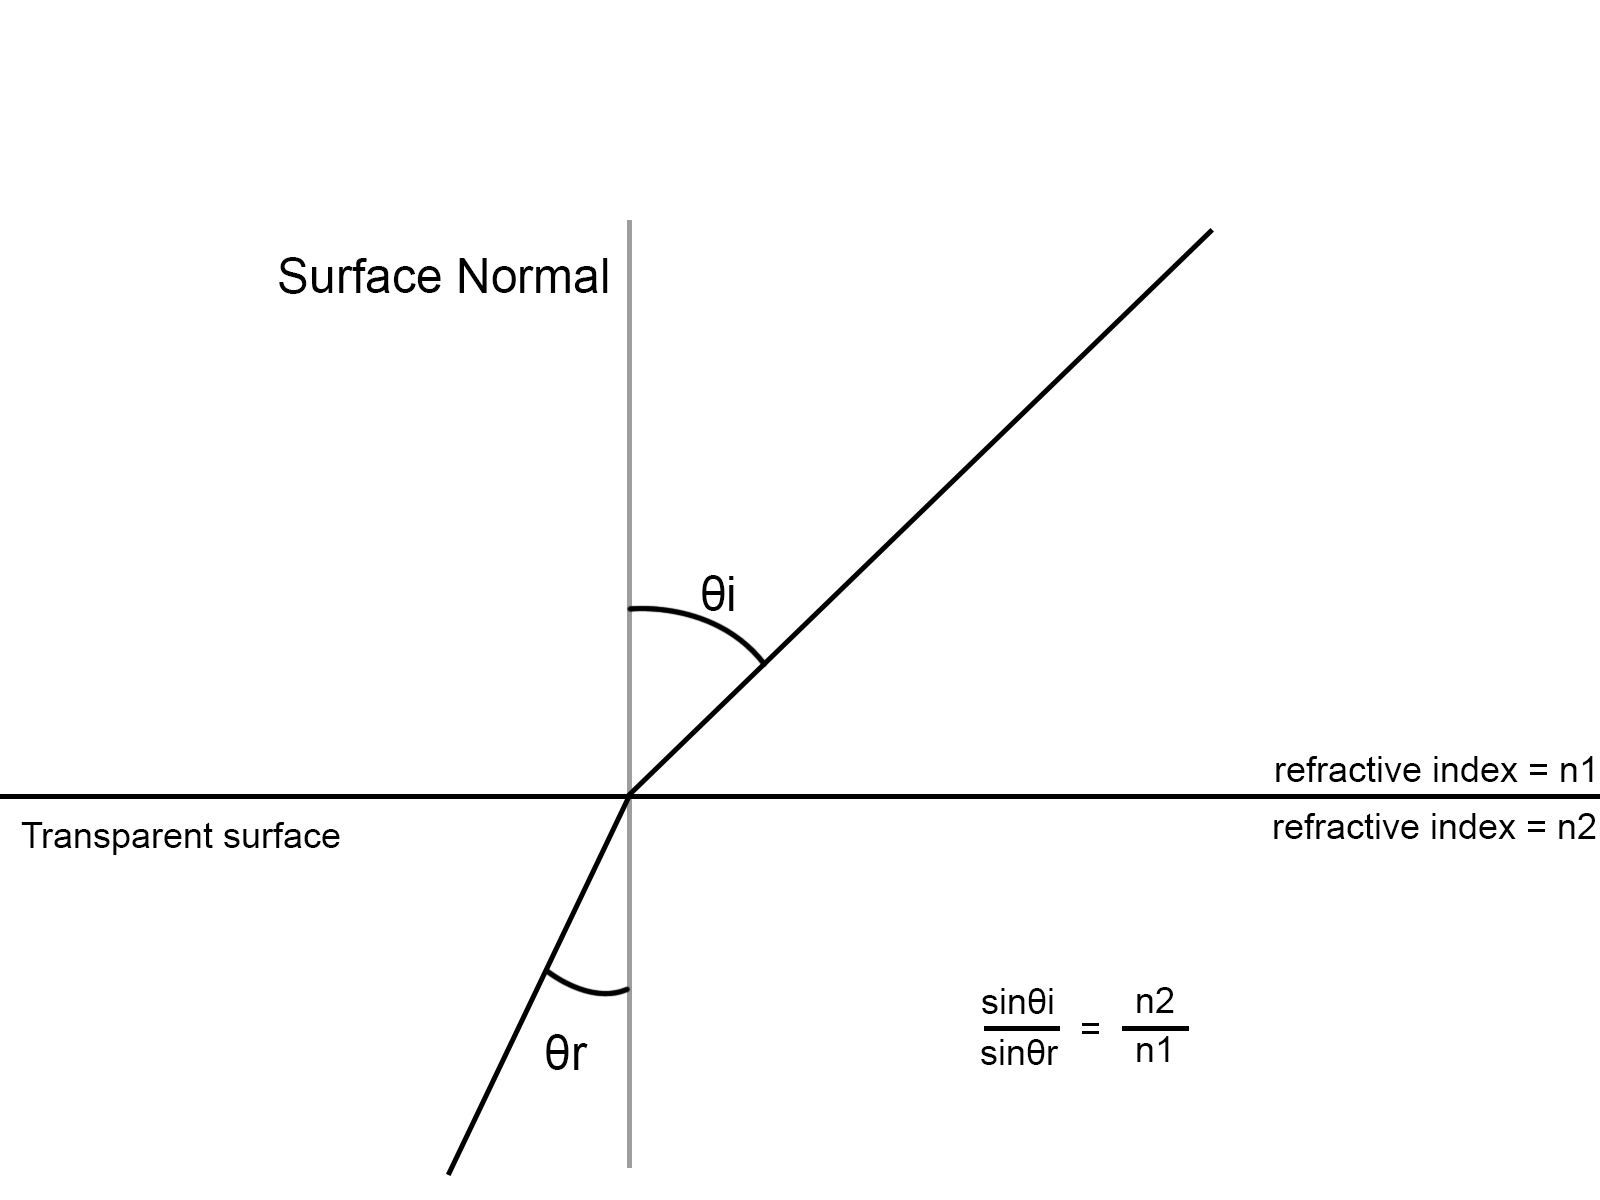
\includegraphics[width=14cm]{refraction.png}
	\caption{The relationship between the angle of incidence $\theta_i$ and the angle of refraction $\theta_r$}
	\label{fig:refraction}
\end{figure}

In order to refract a ray through a surface, the direction of the refracted ray must be calculated. The refracted angle can be calculated by utilising Snell's law, which states a relationship between the angle of incidence $\theta_1$, the angle of refraction $\theta_2$, the index of refraction of the current medium $n1$, and the index of refraction of the medium being entered $n2$ \parencite{glassner89introduction}:

\[
	\frac{\sin\theta_1}{\sin\theta_2} = \frac{n2}{n1}
\]

By using this relationship, it is possible to determine a direction vector for the refracted ray. The GLSL specification again gives a method of calculating a direction vector for a refracted ray, given an incidence vector $I$, a surface normal $N$, and the ratio of the current index of refraction to the new index of refraction $eta$:

\newpage
\lstset{language=C,caption={Calculation of a refraction ray},label=lookuptable}
\begin{lstlisting}[frame=single]
vector refract(vector I, vector N, float eta)
{
	k = 1.0 - eta * eta * (1.0 - dot(N, I) * dot(N, I));

	if (k < 0.0) 
		return vector(0.0, 0.0, 0.0);
	else 
		return eta * I - (eta * dot(N, I) + sqrt(k)) * N;
}
\end{lstlisting}

A refracted ray can then be cast through a material in order to determine the path of light through a medium. When the ray reaches a boundary beyond which the index of refraction changes, the direction of the refraction ray must be recalculated.

One additional consideration must be made, however. The specified normal must be a normal on the plane through which the ray is refracting. In the case of a refraction ray leaving a material, rather than entering it, the normal usually used for rendering a surface will need to be reversed in order to obtain this normal. This can easily be handled by checking the dot product of the normal with the direction of the refracted ray:

\[
	dot = ray.direction \cdot normal
\]

If this dot product is greater than zero, then the surface normal is facing outwards from the direction of the ray, and as such, must be reversed to obtain the normal of the surface through which the ray is being refracted:

\[
	normal = -normal
\]

\subsection{Tracing rays through materials}
In order to handle translucent materials, we must be able to trace a ray through a translucent material. The problem is, given an intersection with a surface, finding the point at which a refraction ray cast from this intersection point exits the surface. One possible solution is to modify the ray casting algorithm, redefining the exit conditions such that it only exits when empty space is found, as in algorithm \ref{alg:raycast_solids}.

\begin{algorithm}
\caption{Ray casting through solids}
\label{alg:raycast_solids}
\begin{algorithmic}[1]
\Procedure{Raycast\_solid}{$root, ray$}
	\State $current\_voxel \gets intersect(root,~ray)$			\Comment{Intersection with root}
	\While{$not~terminated$} \Comment{Traverse}
		\If{$current\_voxel~exists$}
			\State $current\_voxel \gets old\_voxel$
			\State $current\_voxel \gets push(currrent\_voxel, ray)$		\Comment{Descend into child}
		\EndIf

		\State $old\_voxel \gets current\_voxel$
		\State $current\_voxel \gets advance(current\_voxel, ray)$			\Comment{Advance into next sibling}

		\If{$advance~direction~disagrees~with~ray~direction$}
			\State $current\_voxel \gets pop(current\_voxel, old\_voxel)$			\Comment{Pop last common parent}
		\EndIf

		\If{$current\_voxel~nonexistent$}			\Comment{Return when empty space is found}
			\State $\textbf{return}~old\_voxel$
		\EndIf
	\EndWhile
\EndProcedure
\end{algorithmic}
\end{algorithm}

The algorithm will now descend until it finds a leaf node, advancing and popping only once a leaf is found. This algorithm will find the exit point of a ray, but it has the side effect of checking every voxel along the ray's path, at every level. This is very inefficient, and does not take advantage of the volume's tree structure.

On the other hand, if we were to consider the refraction ray discretely, we could follow the path of the ray through the solid, casting back towards the original point of intersection at intervals. Once the active span of the ray as returned by the ray casting algorithm is non-zero, in other words, when the ray has started in empty space and found a surface, we have found the probable exit point of the refraction ray. In order to do this, an interval must be chosen. We chose to use a fixed user-configurable interval, but it may be possible to use a dynamic interval based on the volume being ray traced. The pseudo-code for this operation is given below.

\begin{algorithm}
\caption{Discrete ray cast}
\label{alg:discrete_raycast}
\begin{algorithmic}[1]
\Procedure{Discrete\_raycast}{$root, ray$}
	\State $max\_iterations = \frac{scene\_width}{fixed\_interval}$
	\For{$i = 0;~i<max\_iterations;~++i$}
		\State \Call{Raycast}{origin + i * direction, -direction}
		\If{$resulting~span > 0$} \Comment{We found empty space}
			\State $\textbf{break}$
		\EndIf
	\EndFor
	\State $\textbf{return}~found~surface$
\EndProcedure
\end{algorithmic}
\end{algorithm}

\subsection{Refraction through heterogeneous materials}
It has already been established that the refraction ray's direction must be recalculated when moving from a material with one index of refraction to a material with a different index of refraction. The problem, then, is how to accomplish this for heterogeneous materials.

The above discrete ray cast algorithm can be easily modified to take account of the change in refractive index as it traverses through a material.

\begin{algorithm}
\caption{Discrete ray cast with varying refractive index}
\label{alg:discrete_raycast_heterogeneous}
\begin{algorithmic}[1]
\Procedure{Discrete\_raycast}{$root, ray$}
	\State $max\_iterations = \frac{scene\_width}{fixed\_interval}$
	\State $refractive\_index = hit\_refractive\_index$
	\For{$i = 0;~i<max\_iterations;~++i$}
		\State \Call{Raycast}{origin + i * direction, -direction}
		\If{$resulting~span > 0$} \Comment{We found empty space}
			\State $\textbf{break}$
		\EndIf
		\If{$hit\_refractive\_index != refractive\_index$}
			\If{$\vec{normal} \cdot \vec{direction} > 0$} \Comment{Check if exiting material}
				\State $normal = -normal$
			\EndIf
			\State $direction = \Call{Refract}{direction,~normal,~\frac{refractive\_index}{hit\_refractive\_index}}$
		\EndIf
	\EndFor
	\State $\textbf{return}~found~surface$
\EndProcedure
\end{algorithmic}
\end{algorithm}

\section{Shading}
\begin{figure}
\centering
	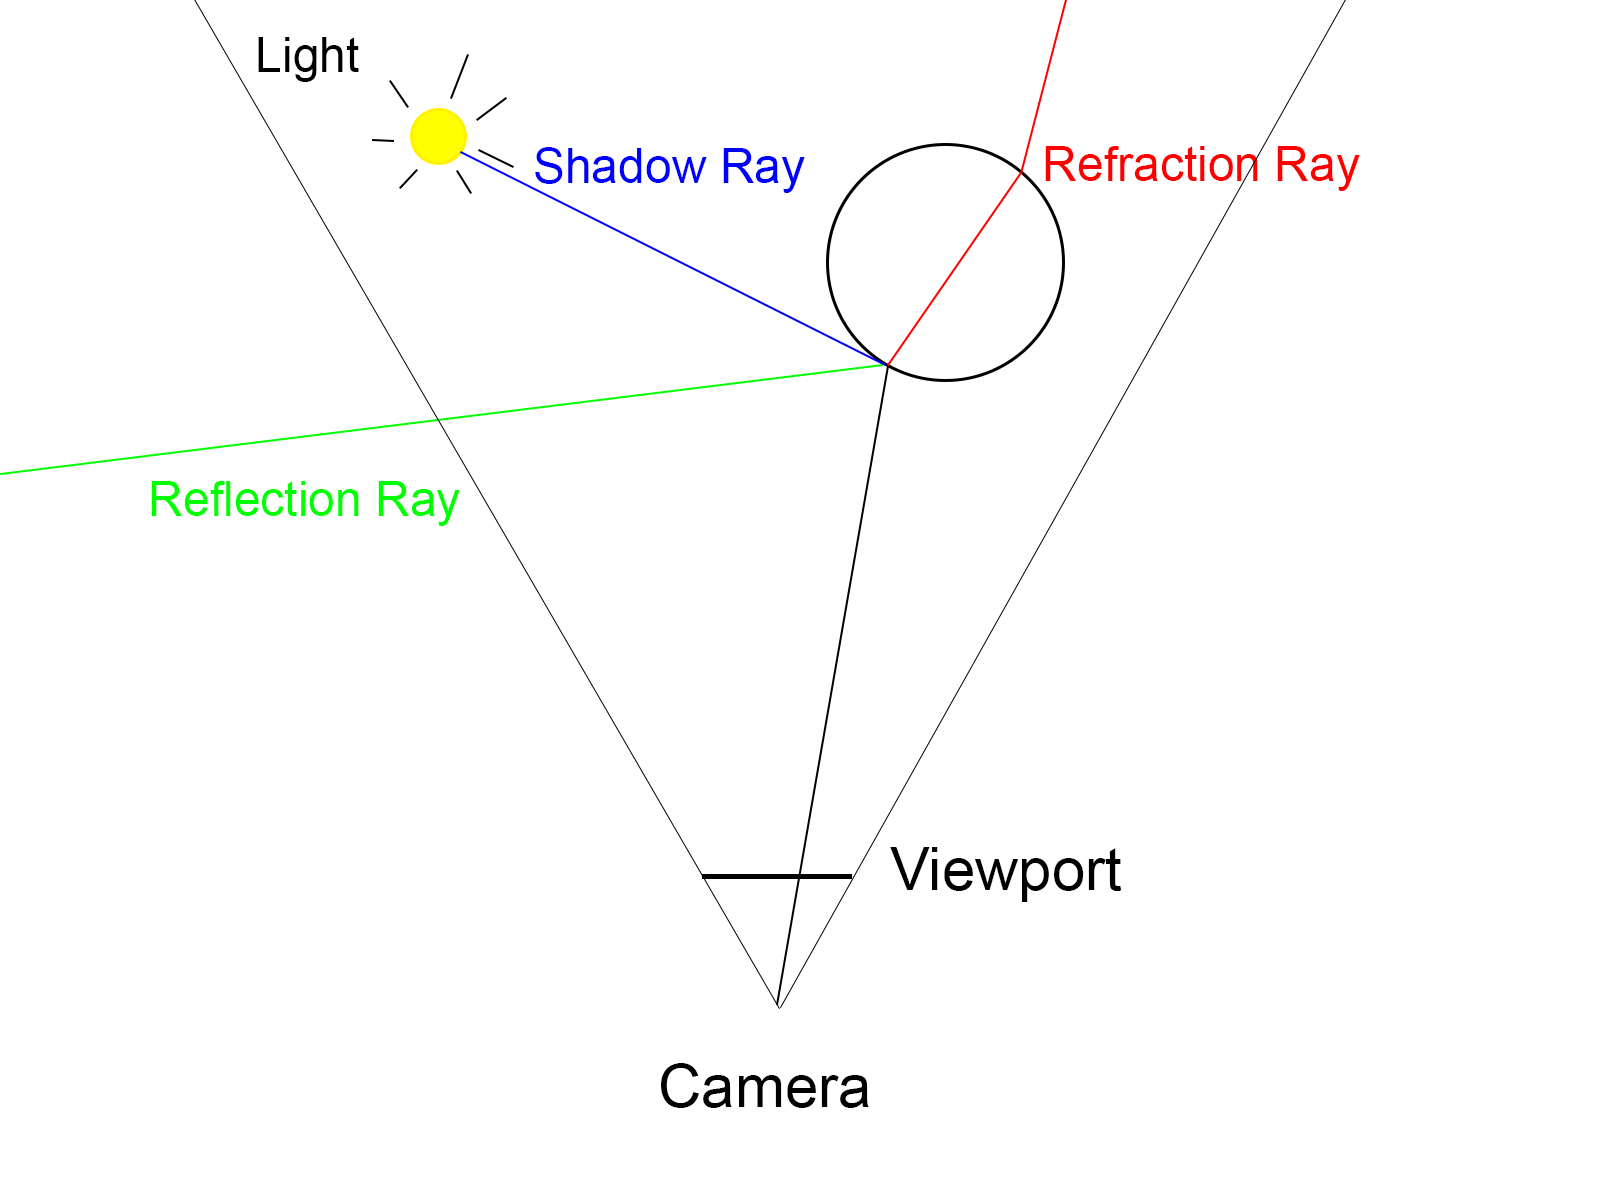
\includegraphics[width=14cm]{secondaryrays.png}
	\caption{Secondary rays being spawned for calculating shadow coverage, reflection, and refraction}
	\label{fig:secondaryrays}
\end{figure}

Our shader uses a Blinn-Phong shading model, as described in chapter \ref{litreview}.

When shading a surface, a ray is cast towards each light source to check if it is occluded, in which case the intersection is in shadow. Reflection and refraction rays are also cast and the results are then mixed additively with the final output colour.

We use recursion to handle multiple levels of reflection and refraction to a predefined maximum. Simplified pseudo-code for rendering and shading is given in algorithm \ref{alg:render}.

\begin{algorithm}
\caption{Per-pixel rendering}
\label{alg:render}
\begin{algorithmic}[1]
\Procedure{render\_pixel}{$x, y, tree, projection$}
	\State $out\_colour \gets (0, 0, 0, 0)$
	\State $ray \gets calculate\_ray(x,~y,~projection)$
	\State $intersection \gets \Call{raycast}{tree, ray}$
	\If{$intersection.hit$}
		\State $out\_colour \gets \Call{shade}{tree,~ ray,~ intersection}$
	\EndIf
	\State $\textbf{return} out_colour$
\EndProcedure
\\
\Procedure{shade}{$tree,~ ray,~ intersection$}
	\State $out\_colour \gets (0, 0, 0, 0)$
	\For{$each~light$} \Comment{Shade for each light}
		\State $light\_dir \gets light\_pos - intersection.position$ \Comment{Check shadow}
		\State $shadow\_ray \gets (intersection.position, light_dir)$
		\State $shadow\_intersection \gets \Call{raycast}{tree, shadow\_ray}$
		\If{$shadow\_intersection.hit$}
			\State $\textbf{continue}$
		\EndIf
		\State $out\_colour ~+=~ \Call{diffuse\_reflection}{intersection,~light}$
		\State $out\_colour ~+=~ \Call{specular\_reflection}{intersection,~light}$
	\EndFor
	\\
	\State $reflection\_ray \gets \Call{reflect}{ray,~intersection}$ \Comment{Reflection}
	\State $reflection\_intersection \gets \Call{raycast}{tree, reflection\_ray}$
	\If{$reflection\_intersection.hit$}
		\State $out\_colour ~+=~ \Call{shade}{tree,~ reflection\_ray,~ reflection\_intersection}$
	\EndIf
	\\
	\State $refraction\_ray \gets \Call{refract}{ray,~intersection}$ \Comment{Refraction}
	\State $refraction\_intersection \gets \Call{raycast\_empty}{tree, refraction\_ray}$
	\If{$refraction\_intersection.hit$}
		\State $out\_colour ~+=~ \Call{shade}{tree,~ refraction\_ray,~ refraction\_intersection}$
	\EndIf
\EndProcedure
\end{algorithmic}
\end{algorithm}

\section{Parallelisation}
Ray tracing is parallelised with one thread per pixel on the screen. This thread is then responsible for the primary ray and all secondary rays, and all work involved in generating that pixel, as shown in algorithm \ref{alg:render}. Pixels are considered independently to allow this process to be parallelised. These threads are spawned on the GPU in 32x32 grids to maximise occupancy. This is the maximum grid size on current generation CUDA GPUs, and allows us to achieve high levels of GPU utilisation as shown in figure \ref{fig:utilisation}.

\begin{figure}
\centering
	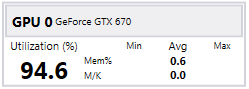
\includegraphics[width=8cm]{gpu0.png}
	\caption{GPU utilisation for our rendering kernel, as determined using Nvidia's nsight profiler}
	\label{fig:utilisation}
\end{figure}

This approach allows us to achieve real-time rendering for simple scenes, and given the results of \cite{laine10efficientsvos} should also allow more complex scenes to be rendered. However, the limitation of this approach is that, as more work is added to each thread, every thread in a grid must follow the most computationally heavy computation path due to the highly parallelised nature of GPUs. Possible solutions to this problem are presented in chapter \ref{conclusion}.

\section{Test data}
Benchmarks for the software were taken by recording the average number of frames per second (FPS) over one minute for a given screen resolution, as well as data resolution. Screen resolution is measured in pixels, while data resolution is measured in nodes of the tree at the lowest level of the tree. This resolution is given by the formula:

\[
	resolution = 2^{max\_scale~ -~ 1}
\]

Such that data generated down to the 11$^{th}$ level has a resolution of $2^{10} = 1024$ in each dimension. This is also referred to as a resolution of $1024^3$.

Each scene has been tested across various screen resolutions as well as data resolutions in order to demonstrate how the algorithms scale with respect to screen ruesolution and data resolution.

In order to evaluate our renderer's performance we have considered the differences in performance for a sample scene with no shadows, reflection or translucency, as screen resolution and data resolution are varied. We consider this data our control sample, and following samples for rendering with shadows, reflection, and translucency is compared with this control.

We have then evaluated the relationships between screen resolution, data resolution, and performance for these samples, as well as compared the overall performance for these samples against our control to determine the effect on performance of considering these effects.

These tests were conducted on a single Nvidia GTX 670.

\section{Implementation}
Our implementation utilises CUDA for all rendering, bypassing the rasterisation process almost entirely. An OpenGL texture is created at program launch, and this texture is then written to by the rendering kernel using OpenGL-CUDA interoperation.

\subsection{OpenGL-CUDA interop}
OpenGL-CUDA interop is accomplished using a pixel buffer object (PBO) that is shared between CUDA and OpenGL. A PBO is stored in GPU memory, eliminating unnecessary copying to main CPU memory. When required by CUDA, the PBO is mapped to a device pointer accessible by cuda, and must be unmapped before it can be accessed again by OpenGL. The PBO can then be unpacked into an OpenGL texture directly, allowing the CUDA-generated buffer to be written to the screen.

A code listing demonstrating how a PBO and a texture are created, and how this PBO is registered with CUDA is available below in code listing \ref{texturecreation}. A code listing for The gpuErrChk macro's code listing is available in appendix \ref{app:cuda-utils}. Once the PBO is created, it can be mapped to a device pointer as shown in code listing \ref{map-buffer}. Once unmapped, its contents can then be unpacked to a texture for display on the screen as demonstrated in \ref{pbo-unpack}. As all of these operations occur directly within GPU memory, unnecessary coping to main memory is avoided.

\subsection{Matrix maths}
Matrix maths is accomplished using GLM, the OpenGL Mathematics library. This is a C++ library which implements all of the features of GLSL and includes CUDA support, making it suitable for writing 3D rendering code and shaders in CUDA.

\newpage
\lstset{language=C,caption={Creation of the OpenGL PBO and texturre},label=texturecreation}
\begin{lstlisting}[frame=single]
void* glFb;

GLuint pbo;
GLuint texid;

// Create pixel buffer object
glGenBuffers(1, &fbo);

// Create buffer texture
glGenTextures(1, &texid);

// Initilaise pixel buffer object with size
glBindBuffer(GL_PIXEL_UNPACK_BUFFER, pbo);
glBufferData(GL_PIXEL_UNPACK_BUFFER,
	viewport.w * viewport.h * 4 * sizeof(GLubyte),
	nullptr, GL_DYNAMIC_DRAW);
glBindBuffer(GL_PIXEL_UNPACK_BUFFER, 0);

// Initialise texture with width, height, and format
glBindTexture(GL_TEXTURE_2D, texid);
glTexImage2D(GL_TEXTURE_2D, 0, GL_RGBA, width, height, 0,
				GL_RGBA, GL_UNSIGNED_BYTE, NULL);
glTexParameteri(GL_TEXTURE_2D, GL_TEXTURE_MAG_FILTER, GL_LINEAR);
glTexParameteri(GL_TEXTURE_2D, GL_TEXTURE_MIN_FILTER, GL_LINEAR);
glBindTexture(GL_TEXTURE_2D, 0);

// Register pixel buffer object with cuda
gpuErrchk(cudaGraphicsGLRegisterBuffer(&glFb, pbo,
			cudaGraphicsRegisterFlagsNone));
\end{lstlisting}

\newpage
\lstset{language=C,caption={Binding the PBO so that CUDA kernels can access it},label=map-buffer}
\begin{lstlisting}[frame=single]

// Bind cuda graphics resources
gpuErrchk(cudaGraphicsMapResources(1, &glFb, 0));

// Get a device pointer to it
gpuErrchk(cudaGraphicsResourceGetMappedPointer(&ptr, &size,
												glFb));

// Pass device pointer to CUDA kernel

// Unmap pbo
gpuErrchk(cudaGraphicsUnmapResources(1, &glFb, 0));
\end{lstlisting}

\lstset{language=C,caption={Unpacking of a PBO to an OpenGL texture},label=pbo-unpack}
\begin{lstlisting}[frame=single]
glBindBuffer(GL_PIXEL_UNPACK_BUFFER, pbo);
glBindTexture(GL_TEXTURE_2D, texid);
glTexEnvi(GL_TEXTURE_ENV, GL_TEXTURE_ENV_MODE, GL_REPLACE);
glTexImage2D(GL_TEXTURE_2D, 0, GL_RGBA, width, height, 0,
				GL_RGBA, GL_UNSIGNED_BYTE, 0);
\end{lstlisting}
\chapter{Implementation}
\label{implementation}

\section{Ray-casting}

\subsection{Contours}

\section{Ray-tracing}

\section{Shading}

\section{Data structure}

\subsection{Generation}

\subsubsection{Sphere}

\subsubsection{Mesh}
\chapter{Results and Analysis}
\label{results}
In line with our objective of creating a real-time GPU ray tracer that is capable of ray tracing heterogeneous translucent materials, there are three main factors to consider when evaluating our work. The first factor is performance. In order to run at real-time frame rates, a minimum performance threshold must be met. The next factor is the size of our data set. The data must be compact enough to fit in GPU memory and still be high resolution enough such that a high quality image can be generated. Additionally, the final image quality must be considered, to determine if the renderer can correctly handle the desired visual effects, and identify any problems with our approach.

\section{Performance}
\label{sec:perf}

\begin{figure}
	\centering
	\subfloat[No effects]{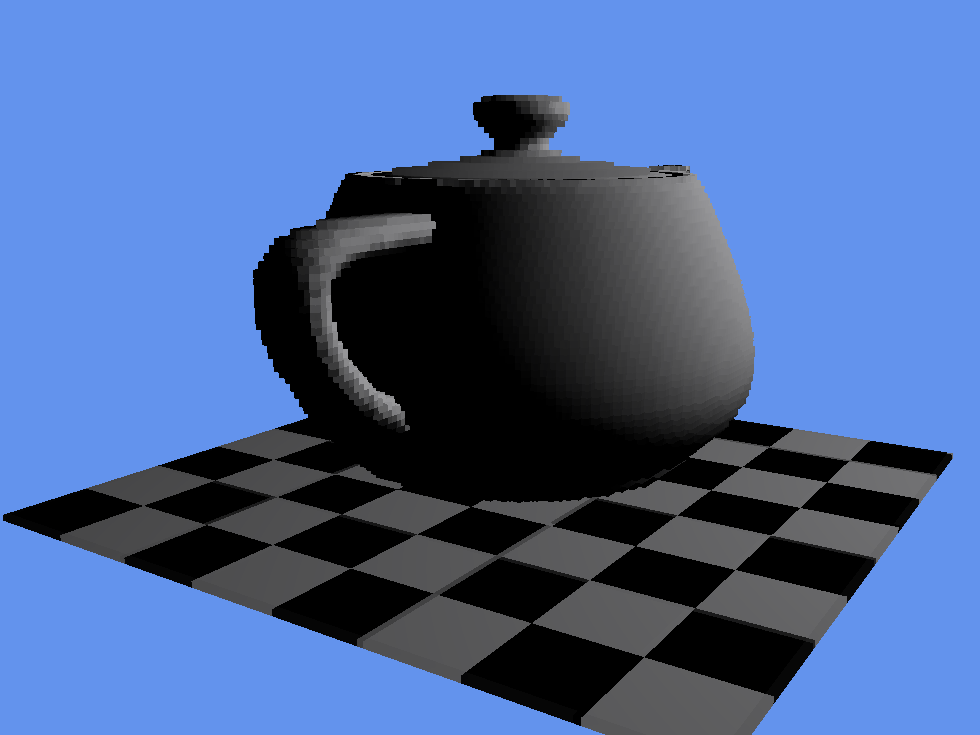
\includegraphics[width=3in]{normal_teapot.png}}
	~
	\subfloat[Shadows]{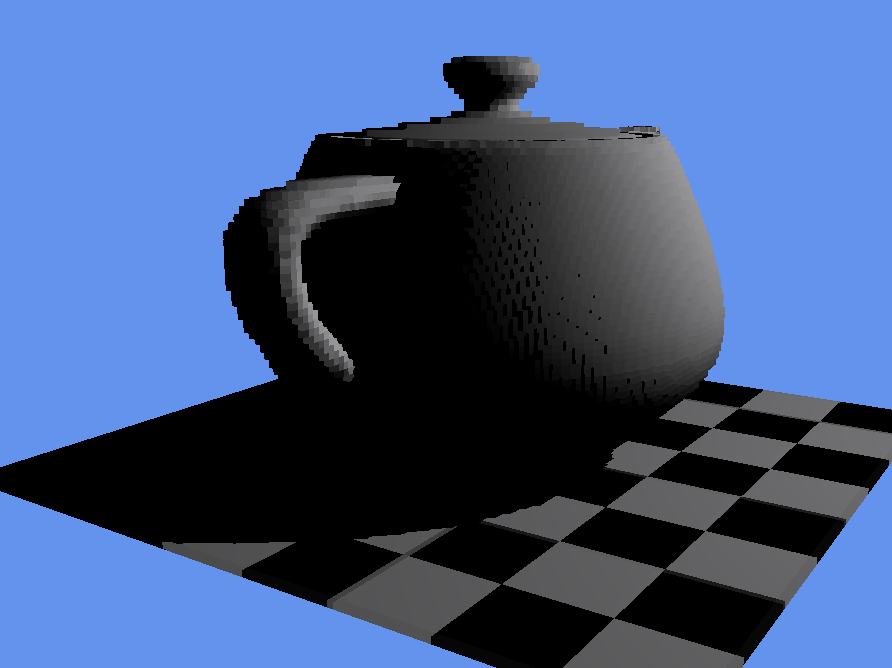
\includegraphics[width=3in]{shadow_teapot.png}}
	\\
	\subfloat[Reflection]{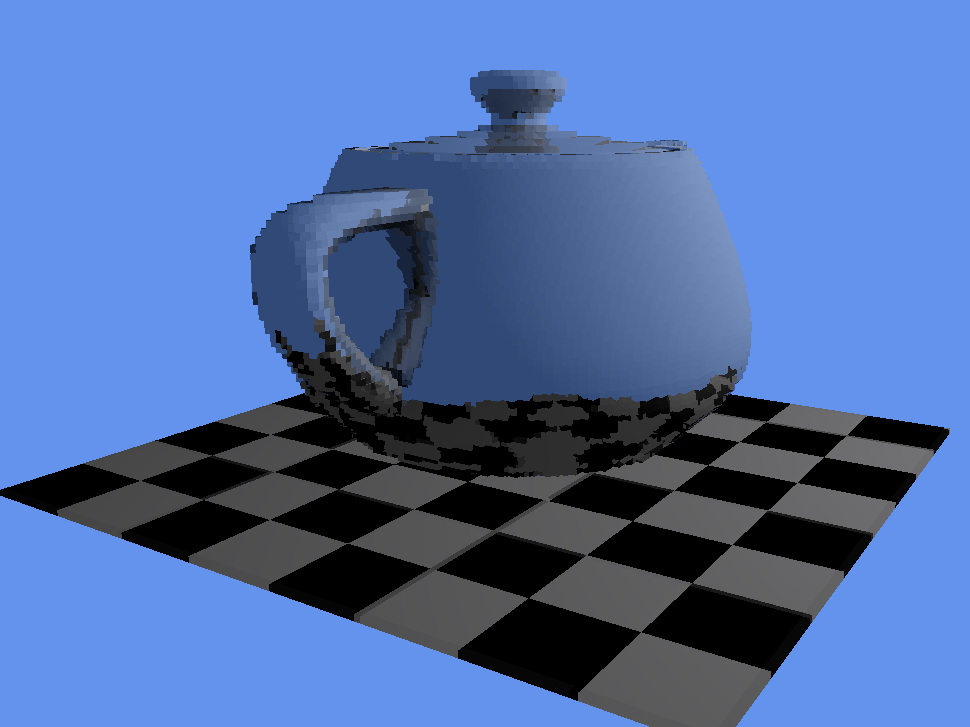
\includegraphics[width=3in]{reflective_teapot.png}}
	~
	\subfloat[Translucency]{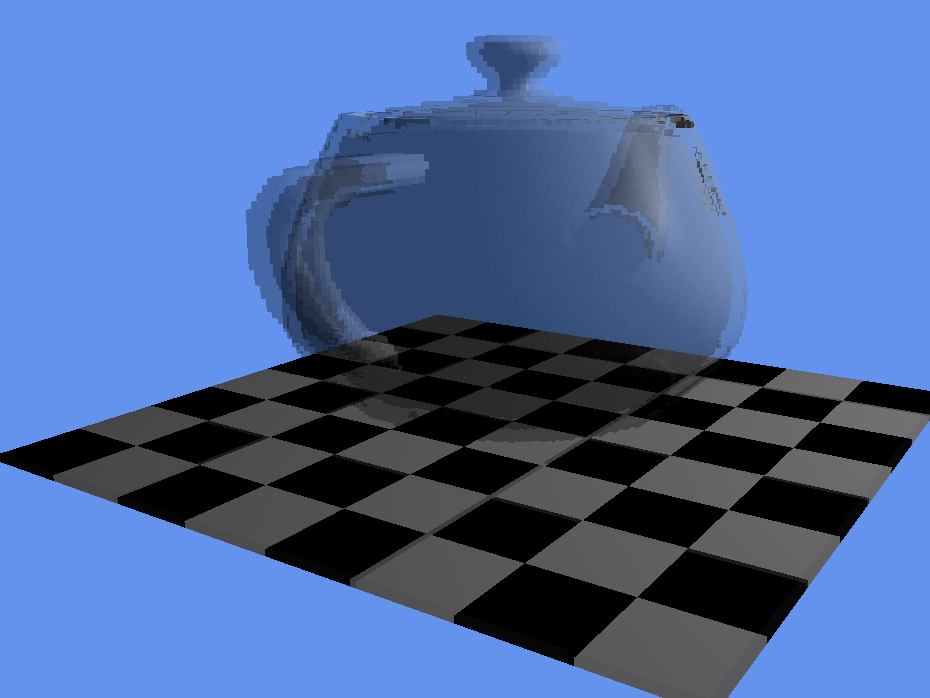
\includegraphics[width=3in]{translucent_teapot.png}}

	\caption{Our test scene at a $512^3$ resolution with various options turned on}
	\label{fig:performance-data}
\end{figure}

In evaluating the performance of our renderer there are three main criteria to consider: that it can produce reasonable quality images in real-time at high screen resolutions; that it scales well with the resolution of the data, such that the overall quality of the image produced is comparable to that of rasterisation-based renderers; and that it scales well with the resolution of the screen, such that it can be used at the higher screen resolutions desired for games.

Figure \ref{fig:performance-data} shows the resulting image from our sample scene at $512^3$ resolution with each effect enabled.

\subsection{Table of results}
\vspace{1em}

\begin{tabular}{|l|r|r|r|}
\hline

Scene \hspace{200pt} & Screen Res & Data Res & Avg FPS \\
\hline

	\quad 1 \quad		Teapot							& 768x768		& $512^2 $	&	99.34	\\
		\cline{3-4}
	\quad \quad \quad	on checker board plane			& 				& $1024^2 $	&	85.17	\\
	\cline{3-4}
														&				& $2048^2 $ &	71.55	\\
		\cline{2-4}
														& 1024x1024		& $512^2 $	&	63.05	\\
		\cline{3-4}
														& 				& $1024^2 $	&	54.45	\\
	\cline{3-4}
														&				& $2048^2 $ &	46.09	\\
		\cline{2-4}
														& 1920x1080		& $512^2 $	&	31.18	\\
		\cline{3-4}
														& 				& $1024^2 $	&	26.38	\\
	\cline{3-4}
														&				& $2048^2 $ &	22.68	\\
\hline

	\quad 2 \quad		Teapot with shadow				& 768x768		& $512^2 $	&	77.46	\\
		\cline{3-4}
	\quad \quad \quad	on checker board plane			& 				& $1024^2 $	&	65.32	\\
	\cline{3-4}
														&				& $2048^2 $ &	55.22	\\
		\cline{2-4}
														& 1024x1024		& $512^2 $	&	49.54	\\
		\cline{3-4}
														& 				& $1024^2 $	&	42.04	\\
	\cline{3-4}
														&				& $2048^2 $ &	36.10	\\
		\cline{2-4}
														& 1920x1080		& $512^2 $	&	23.24	\\
		\cline{3-4}
														& 				& $1024^2 $	&	19.40	\\
	\cline{3-4}
														&				& $2048^2 $ &	16.89	\\
\hline

	\quad 3 \quad		Reflective teapot				& 768x768		& $512^2 $	&	69.83	\\
		\cline{3-4}
	\quad \quad \quad	on checker board plane			& 				& $1024^2 $	&	58.64	\\
	\cline{3-4}
														&				& $2048^2 $ &	49.13	\\
		\cline{2-4}
														& 1024x1024		& $512^2 $	&	46.68	\\
		\cline{3-4}
														& 				& $1024^2 $	&	37.99	\\
	\cline{3-4}
														&				& $2048^2 $ &	31.93	\\
		\cline{2-4}
														& 1920x1080		& $512^2 $	&	20.44	\\
		\cline{3-4}
														& 				& $1024^2 $	&	16.88	\\
	\cline{3-4}
														&				& $2048^2 $ &	14.18	\\
\hline

	\quad 4 \quad		Translucent teapot				& 768x768		& $512^2 $	&	39.48	\\
		\cline{3-4}
	\quad \quad \quad	on checker board plane			& 				& $1024^2 $	&	32.32	\\
	\cline{3-4}
														&				& $2048^2 $ &	25.25	\\
		\cline{2-4}
														& 1024x1024		& $512^2 $	&	24.38	\\
		\cline{3-4}
														& 				& $1024^2 $	&	20.11	\\
	\cline{3-4}
														&				& $2048^2 $ &	15.96	\\
		\cline{2-4}
														& 1920x1080		& $512^2 $	&	10.07	\\
		\cline{3-4}
														& 				& $1024^2 $	&	8.30	\\
	\cline{3-4}
														&				& $2048^2 $ &	6.14	\\
\hline
\end{tabular}

\subsection{Real-time rendering}
For the purposes of our evaluation, we are defining real-time as above 30 frames per second. This is not only the minimum frame rate at which a game is expected to run, but is also above the minimum of approximately 20 required for smooth motion. Ideally, 60 frames per second is desired, as this is the refresh rate of most desktop monitors, as well as a common frame rate at which games are expected to run.

To determine if these thresholds are being met, we measure frame rate over one minute and average it.

\subsection{Scaling with screen resolution}
Our renderer is expected to perform at the high resolutions demanded by games. As our render is parallelised per pixel, in order to test how well this parallelisation functions, we have taken measurements for three screen resolutions: 768x768 (approximately 550k pixels,) 1024x1024 (approximately 1000k pixels,) and 1920x1080 (approximately 2000k pixels.) 1920x1080 was chosen as our benchmark resolution as it is at the upper bounds of standard display resolutions for video games, and as such, our renderer should be able to handle it. The lower resolutions were chosen due to an approximate doubling of pixels between each one, and as such it should allow us to determine whether our performance scales well with screen resolution.

\subsection{Scaling with data resolution}
A 3D renderer must be able to handle data of a resolution high enough to display the data smoothly. For this reason, we have chosen to measure the performance at varying data resolutions in order to determine how our methods scale with the resolution of the data.

 A $1024^3$ resolution (1024 subdivisions in each axis) was chosen as this is the resolution needed to show our data up close with similar quality to a rasterisation-based renderer. Samples were also taken at $2048^3$ and $512^3$ resolutions in order to determine how the performance is affected by varying data resolutions.

\subsubsection{Rendering with no effects (control)}
\begin{figure}[H]
\centering
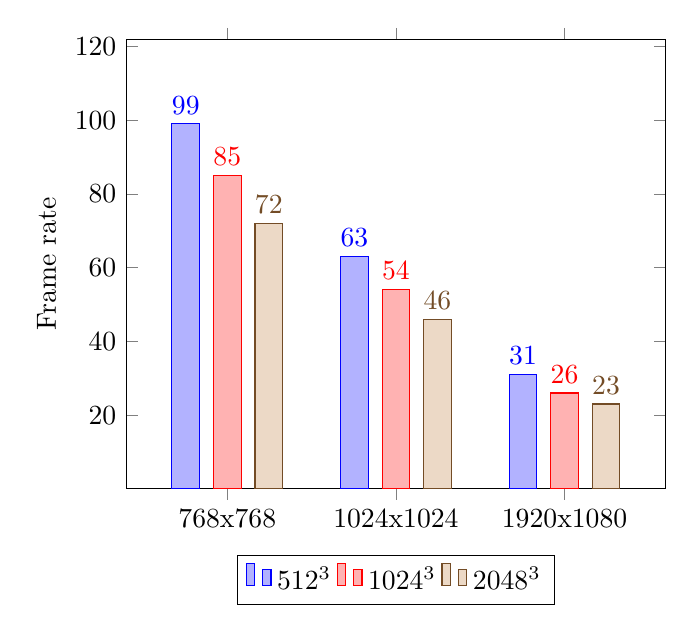
\begin{tikzpicture}
\begin{axis}[
    ybar=5pt,
    enlargelimits=0.3,
    legend style={at={(0.5,-0.15)},
      anchor=north,legend columns=-1},
    ylabel={Frame rate},
    symbolic x coords={768x768,1024x1024,1920x1080},
    xtick=data,
    nodes near coords,
    nodes near coords align={vertical},
    ]
\addplot coordinates {(768x768,99) (1024x1024,63) (1920x1080,31)}; % 512^3
\addplot coordinates {(768x768,85) (1024x1024,54) (1920x1080,26)}; % 1024^3
\addplot coordinates {(768x768,72) (1024x1024,46) (1920x1080,23)}; % 2048^3
\legend{$512^3$,$1024^3$,$2048^3$}
\end{axis}
\end{tikzpicture}

\caption{A plot of frame rate against screen resolution for our control}
\end{figure}

This data functions as our control sample, and allows us to analyse the effect on performance that different visual effects have. By examining the differences in performance with this mode of rendering, and considering the averages and ranges of these differences in performance, we can determine exactly what is affecting performance.

As shown by the graph above, our renderer exhibits a decrease in performance as the number of pixels on the screen is increased. The number of pixels increases by 78\% from 768x768 to 1024x1024, with performance decreasing by 36.0\% on average with a range of 0.94\%. For a linear decrease, one would expect the performance to increase by $100 (1 -\frac{1}{1.78}) = 44\%$, meaning that our parallelisation results in a slightly better than linear decrease in performance when the number of pixels on the screen are increased.

On the other hand, the number of pixels from 1024x1024 to 1920x1080 increases by 98\%, with performance decreasing by an average of 51.0\%, with a range of just 0.25\%. In other words, with the number of pixels on the screen doubled, the performance halves, meaning that, at high screen resolutions such as these, the performance increases linearly.

This is disappointing, and highlights a weakness in our parallelisation scheme. At higher resolutions, our renderer drops down to and below the lower end of our desired threshold for real-time rendering. With better parallelisation, one would expect a less than linear decrease in performance, with a perfectly parallelised process operating in constant time when the number of pixels is varied.

On the other hand, rendering appears to scale well with data resolution. As the resolution of the data is increased by 8 times at each step, the performance decreases by an average of 14.7\% between steps, with an average range of only 1.6\%. As such, the data structure performs very well, and should allow the rendering of a range of scenes of varying resolutions.

\subsubsection{Rendering with shadows}
\begin{figure}[H]
\centering
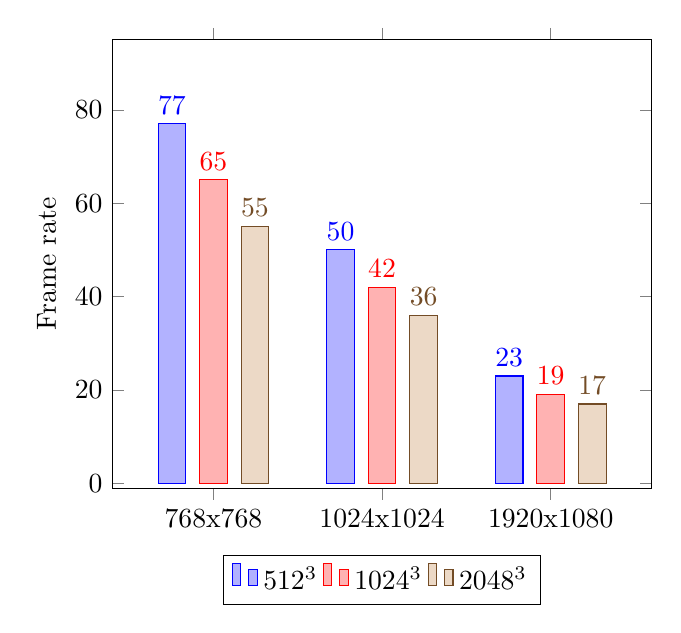
\begin{tikzpicture}
\begin{axis}[
    ybar=5pt,
    enlargelimits=0.3,
    legend style={at={(0.5,-0.15)},
      anchor=north,legend columns=-1},
    ylabel={Frame rate},
    symbolic x coords={768x768,1024x1024,1920x1080},
    xtick=data,
    nodes near coords,
    nodes near coords align={vertical},
    ]
\addplot coordinates {(768x768,77) (1024x1024,50) (1920x1080,23)}; % 512^3
\addplot coordinates {(768x768,65) (1024x1024,42) (1920x1080,19)}; % 1024^3
\addplot coordinates {(768x768,55) (1024x1024,36) (1920x1080,17)}; % 2048^3
\legend{$512^3$,$1024^3$,$2048^3$}
\end{axis}
\end{tikzpicture}

\caption{A plot of frame rate against screen resolution for rendering with shadows}
\end{figure}

As shown by the graph above, the same relationships are seen when shadows are enabled, with a minor decrease in performance. Shadow rays decrease performance by an average of 23.5\%, with a range of just 5.0\% between varying screen resolutions and data resolutions.

The range in performance decrease as screen resolution is varied ranges from 1.0\% to 1.3\%, while the same range for varying data resolutions is 3.6\% to 4.0\%, implying that data resolution is the major contributor to shadow performance. This makes sense, as the only difference between our control and shadow rendering (with reflection turned off, at least) is that a single extra ray per pixel is cast through the data. Despite this, the difference is very low, allowing the same relationships as in the control samples to show through.

Despite this decrease in performance, the performance still scales as well as the performance in our control samples, meaning that the major factors in scaling should still be the same factors as those for our control.

\subsubsection{Rendering with reflection}
\begin{figure}[H]
\centering
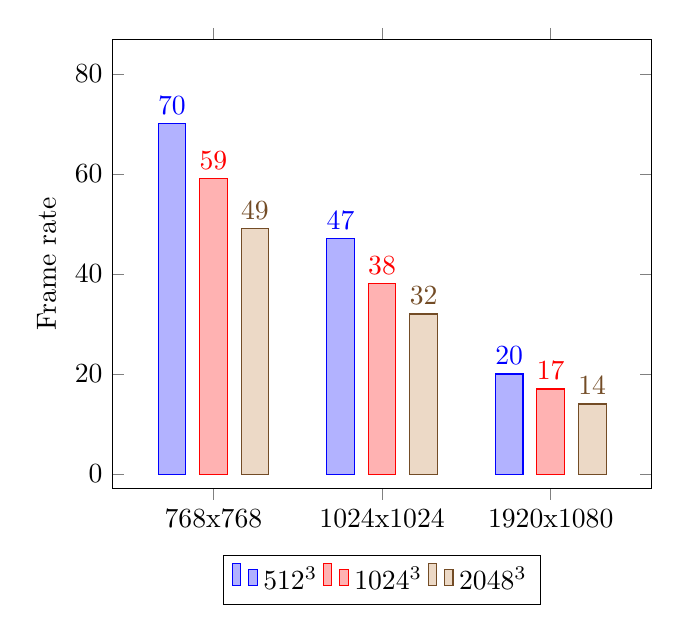
\begin{tikzpicture}
\begin{axis}[
    ybar=5pt,
    enlargelimits=0.3,
    legend style={at={(0.5,-0.15)},
      anchor=north,legend columns=-1},
    ylabel={Frame rate},
    symbolic x coords={768x768,1024x1024,1920x1080},
    xtick=data,
    nodes near coords,
    nodes near coords align={vertical},
    ]
\addplot coordinates {(768x768,70) (1024x1024,47) (1920x1080,20)}; % 512^3
\addplot coordinates {(768x768,59) (1024x1024,38) (1920x1080,17)}; % 1024^3
\addplot coordinates {(768x768,49) (1024x1024,32) (1920x1080,14)}; % 2048^3
\legend{$512^3$,$1024^3$,$2048^3$}
\end{axis}
\end{tikzpicture}

\caption{A plot of frame rate against screen resolution for rendering with reflection}
\end{figure}

Similarly to rendering with shadows, this data exhibits the same relationships as our control. This time, the average decrease in performance is 32.0\%, with a much greater overall range of 11.5\%. The performance decrease ranges from 1.6\% to 4.8\% as the screen resolution is increased, while ranging from 5.8\% to 8.5\% as data resolution is varied, indicating that, again, data resolution is the major factor affecting differences in performance of reflection.

Despite this, these ranges are still minor compared to the average difference, allowing the data to still show similar relationships to those shown by the control data.

Additionally, the performance does not seem to decrease significantly as data resolution is increased.

\subsubsection{Rendering with translucency}
\begin{figure}[H]
\centering
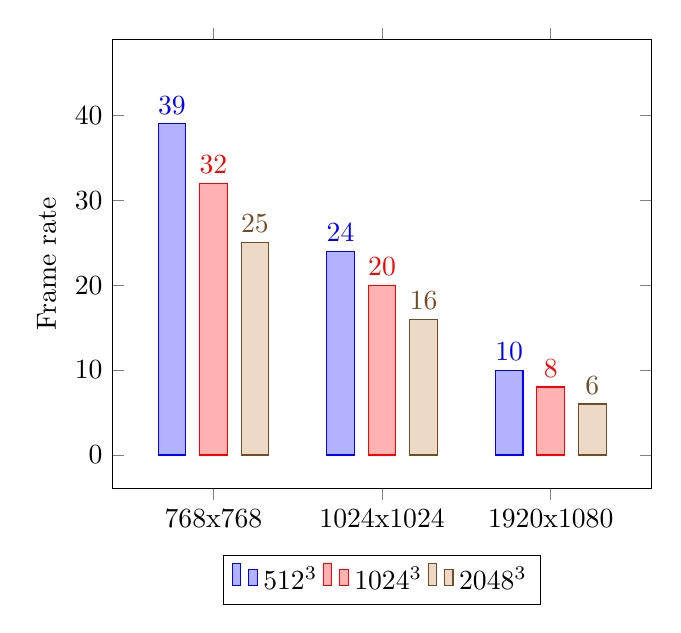
\begin{tikzpicture}
\begin{axis}[
    ybar=5pt,
    enlargelimits=0.3,
    legend style={at={(0.5,-0.15)},
      anchor=north,legend columns=-1},
    ylabel={Frame rate},
    symbolic x coords={768x768,1024x1024,1920x1080},
    xtick=data,
    nodes near coords,
    nodes near coords align={vertical},
    ]
\addplot coordinates {(768x768,39) (1024x1024,24) (1920x1080,10)}; % 512^3
\addplot coordinates {(768x768,32) (1024x1024,20) (1920x1080,8)}; % 1024^3
\addplot coordinates {(768x768,25) (1024x1024,16) (1920x1080,6)}; % 2048^3
\legend{$512^3$,$1024^3$,$2048^3$}
\end{axis}
\end{tikzpicture}

\caption{A plot of frame rate against screen resolution for rendering with translucency}
\end{figure}

This data also exhibits the same relationships as our control, but the reduction in performance is far greater when compared to shadows and reflection. The average reduction in performance for rendering our translucent object was 65.1\%, with an overall range close to that of reflection at 12.7\%. The range for varying screen resolution was 4.0\% - 5.2\%, while the range for varying data resolution was 5.5\% - 8.2\%. These are, again, not a major problem, as the data still exhibits similar relationships to the control data.

Despite this, the data for translucency shows a good relationship between performance and data resolution, with rendering scaling well as data resolution is increased. This makes sense, as our method of determining translucency is discrete, meaning it considers the volume at discrete, fixed intervals rather than the resolution of the data.

The overall decrease in performance, however, is an issue, with performance at 1920x1080 dropping into single digits. Even at lower resolutions, the performance dips below real-time frame rates.

We believe the decrease in performance comes from adding more work to the thread that renders each pixel. As more work is added to the thread, every thread must follow the most computationally expensive execution path due to the SIMD nature of the GPU. In order to address this, we believe that investigation into alternate parallelisation schemes is required.

The persistent threads technique demonstrated in \cite{aila2009hpg} seems like it could improve the parallelisation of our renderer. Firstly, the number of threads spawned on a GPU is related to achieving maximum occupancy on that GPU rather than the number of pixels on the screen, which we have shown to drop off in performance gains at higher resolutions. 

Additionally, as the processes for the initial intersection with the volume, shadows, reflection and refraction all require casting rays within the volume, we believe that it may be possible to create persistent threads that can handle any of these operations, rather than having one thread that handles all of them.

\section{Memory usage}
\label{sec:memusage}
Memory usage is an important factor to consider in real-time rendering. Ideally, all required data should be compact enough to be stored in memory. Even if this is not the case, it is desired for the memory usage to be as low as possible to reduce the amount of memory that must be considered for streaming. In order to evaluate memory usage, we have looked at the memory usage of our test scenes from section \ref{sec:perf}. Our data structure encodes volume data as well as shading data, which must be taken into account when analysing this data.

Figure \ref{fig:memory_usage} shows the memory usage of our test scene at each resolution.

\begin{figure}[H]
	\centering
	\subfloat[$512^3$ resolution, memory usage 34,354kB]{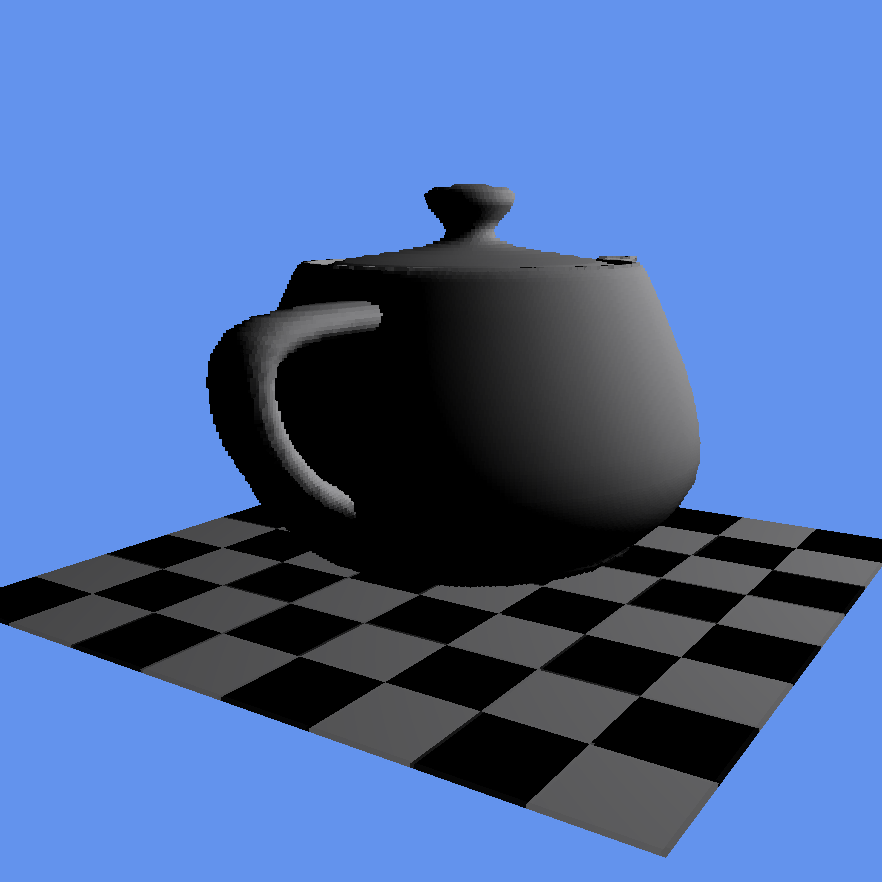
\includegraphics[width=3in]{512cubed_teapot.png}}
	~
	\subfloat[$1024^3$ resolution, memory usage 137,141kB]{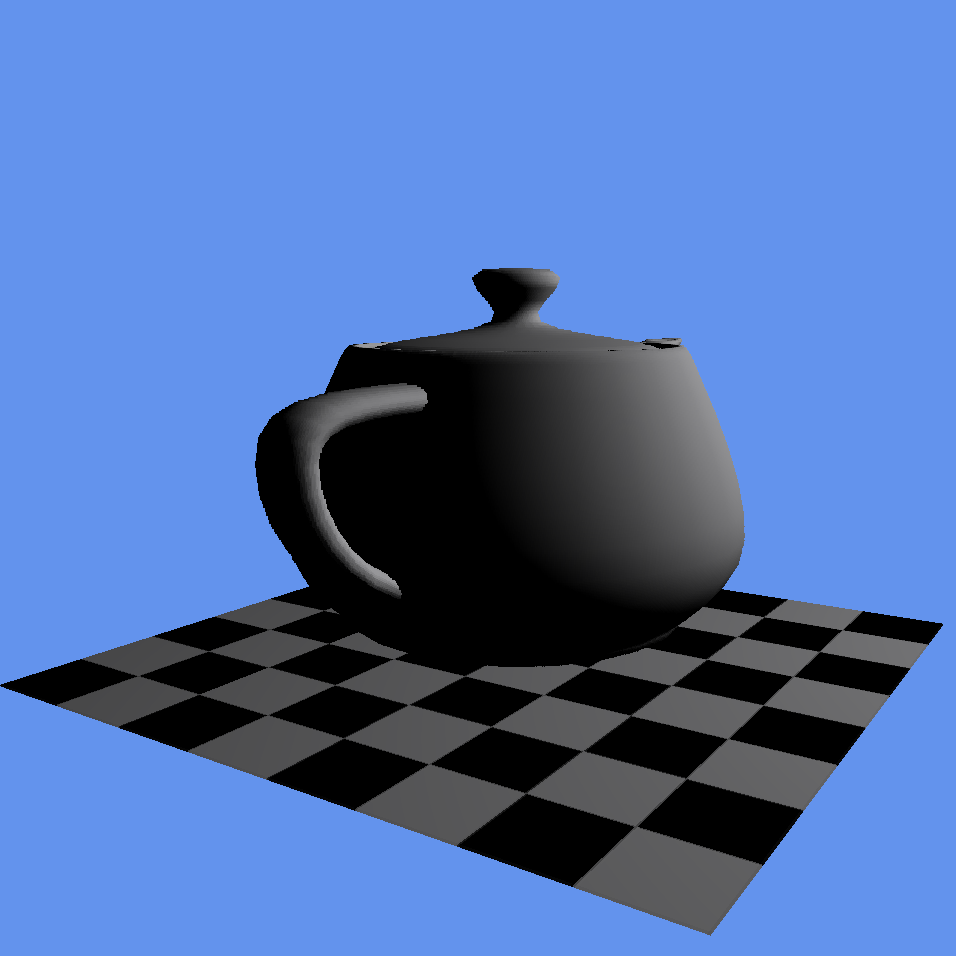
\includegraphics[width=3in]{1024cubed_teapot.png}}
	\\
	\subfloat[$2048^3$ resolution, memory usage 543,832kB]{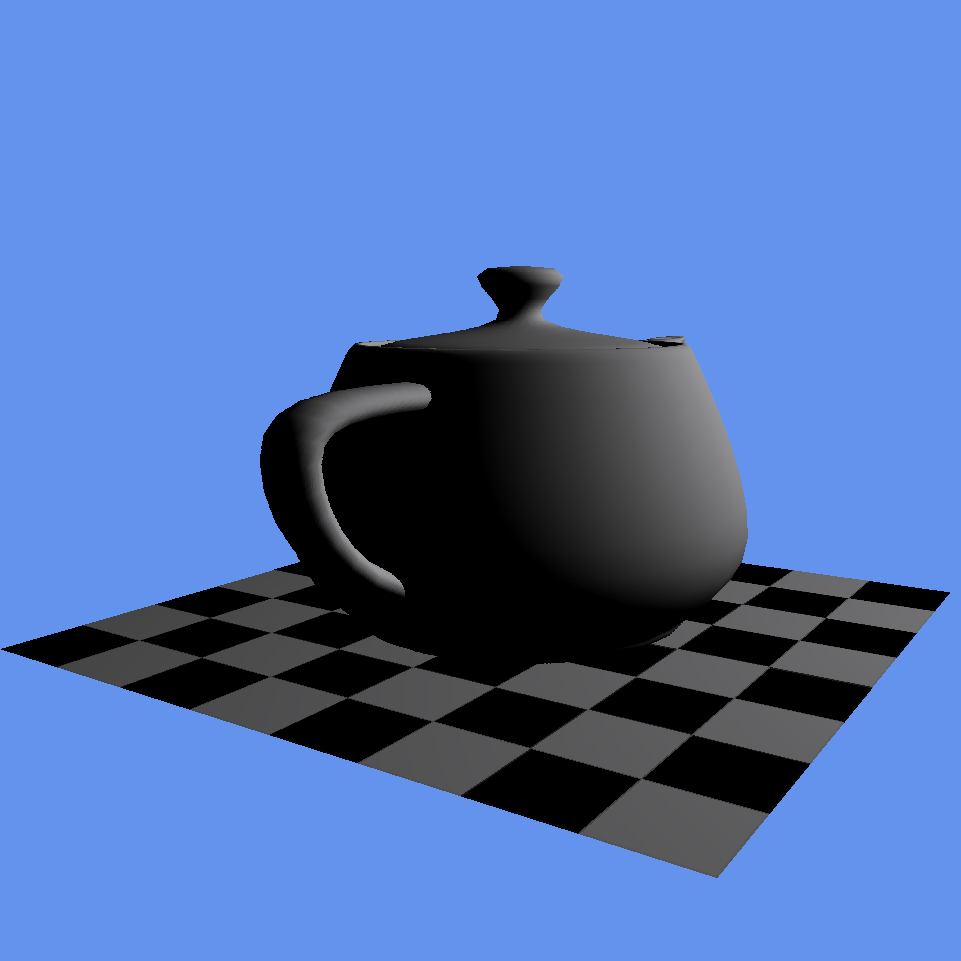
\includegraphics[width=3in]{2048cubed_teapot.png}}

	\caption{Our test scene at various resolutions and the resulting memory usage}
	\label{fig:memory_usage}
\end{figure}

As can be seen, the memory usage increases significantly for every power-of-two increase in resolution. In practice, a $1024^3$ resolution is often sufficient for smooth rendering, however up close, greater resolutions may be required. Despite the structure being compact enough to fit into GPU memory for our example scene, the memory usage is significantly greater than polygon-based meshes. Despite this structure including both volume and shading data, it still has unsatisfactorily high memory usage.

Two major approaches have been been suggested by other works to reduce the memory usage of the sparse voxel octree: contours \parencite{laine10efficientsvos}, which utilise non-cubical voxels to increase the approximation of the original data, removing the need for deeper encoding once the approximation becomes sufficient; and sparse voxel DAGs \parencite{kampe2013dags}, which allow identical regions to share pointers, and can reduce the memory usage of such structures by one to three orders of magnitude. Despite the high memory usage of our structure, these techniques should also be applicable to our work.

\section{Image quality}

\subsection{Accuracy of heterogeneous refraction}
In order to test the accuracy of our method of calculating heterogeneous refraction, we utilise two sets of data: a sphere with refractive index 1.5, with a hollow half-radius sphere embedded in it (see figure \ref{fig:half-radius-sphere}); and a sphere with refractive index 1.5, with a half-radius sphere embedded inside it of refractive index 1.0. In theory, as the refractive index of air is considered to be 1.0, the resulting images should be identical.

\begin{figure}
	\centering
	\subfloat[]{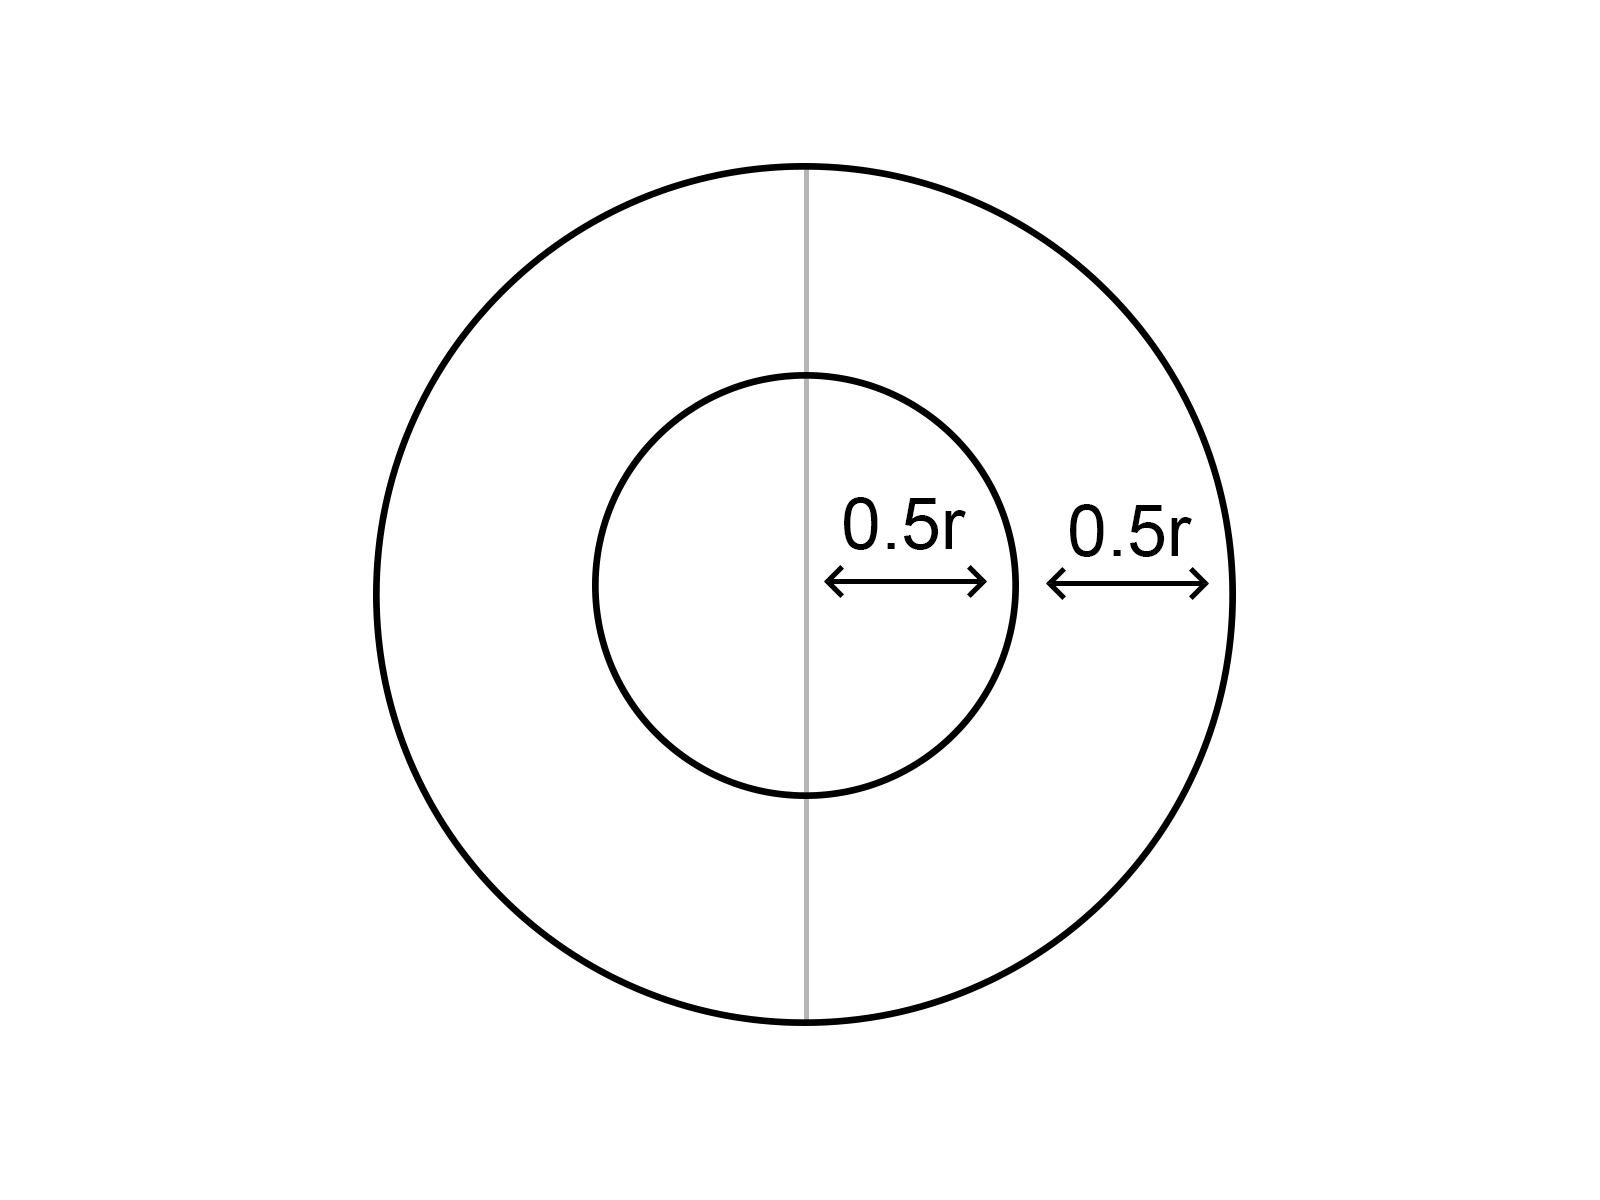
\includegraphics[width=4in]{half-radius.PNG}}

	\caption{A 2D cross section of the sphere used in this experiment. In one data set, the centre is hollow. In the other, it has a refractive index of 1.0}
	\label{fig:half-radius-sphere}
\end{figure}

\begin{figure}
	\centering
	\subfloat[Hollow centre]{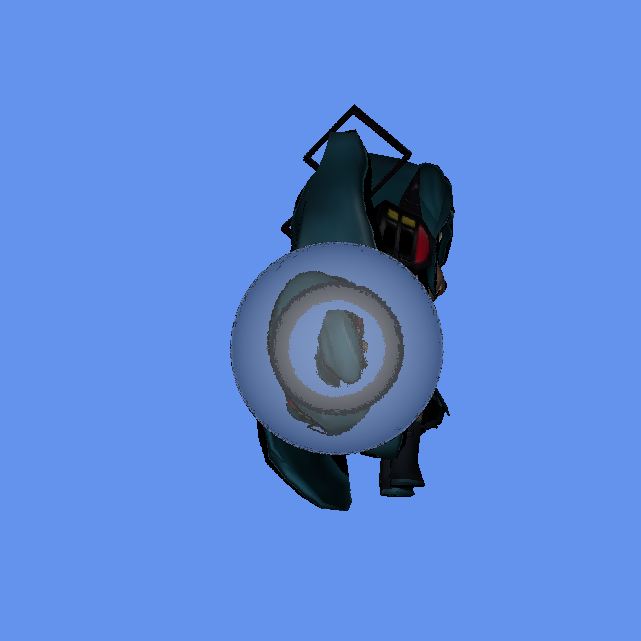
\includegraphics[width=3in]{mikuhollow.png}}
	~
	\subfloat[Refractive index 1 centre]{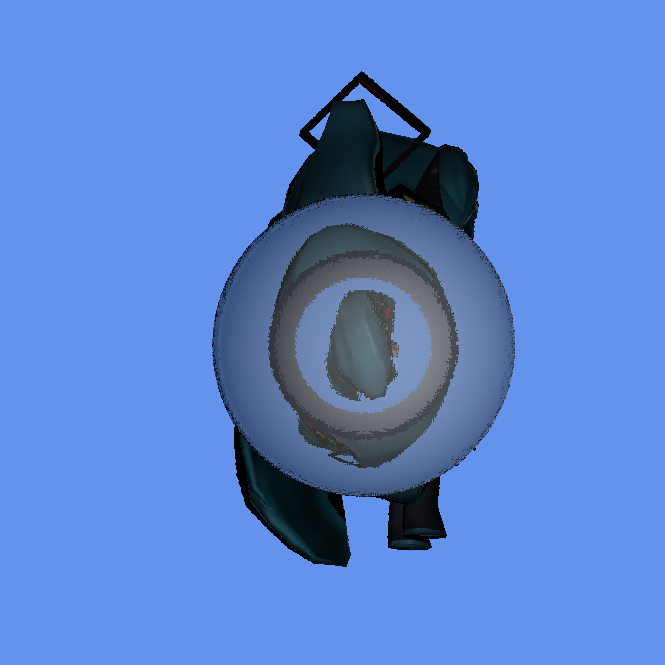
\includegraphics[width=3in]{mikunothollow.png}}

	\caption{The resulting images are identical}
	\label{fig:heterogeneous_refraction}
\end{figure}

As can be seen in figure \ref{fig:heterogeneous_refraction}, our heterogeneous refraction works as intended. It is important to note, however, that this does not prove that the result is physically accurate. Further work is required, comparing the output of our renderer to real objects that exhibit varying indices of refraction, in order to determine its physical correctness.

\subsection{Issues due to the cubical nature of voxel data}

\begin{figure}
	\centering
	\subfloat[A voxel approximation of a cube]{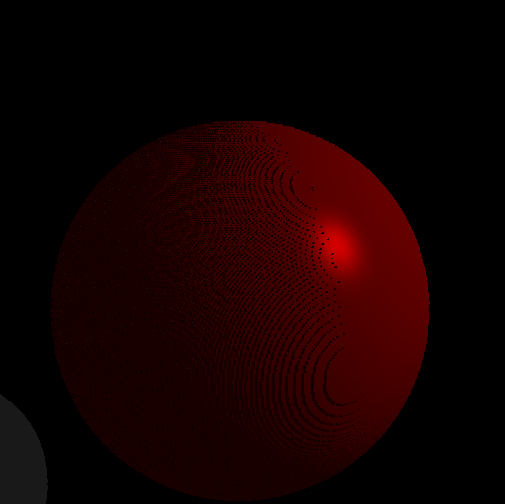
\includegraphics[width=2in]{shadowproblem.png}}
	~
	\subfloat[The phenomenon up close]{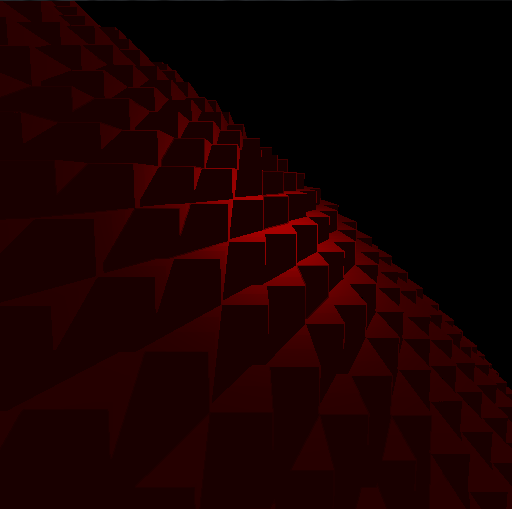
\includegraphics[width=2in]{supersmoothcube.png}}

	\caption{A voxel approximation of a cube casting shadows on itself}
	\label{fig:shadow-problem}
\end{figure}

As can be seen in figure \ref{fig:shadow-problem}, the cubical nature of voxels poses a great issue when considering secondary rays. As a sphere is a convex shape, it should, in theory, be unable to cast any shadows on its own surface. Despite this, the voxel approximation of a sphere casts shadows on itself, causing unsightly black artifacts. This problem generalises to any curved surface, as well as other types of secondary rays, such as reflection and refraction rays. Figure \ref{fig:shadow-problem-ray-path} demonstrates why this occurs, by considering the path of a shadow ray from part of the surface that is in shadow.

\begin{figure}
	\centering
	\subfloat[]{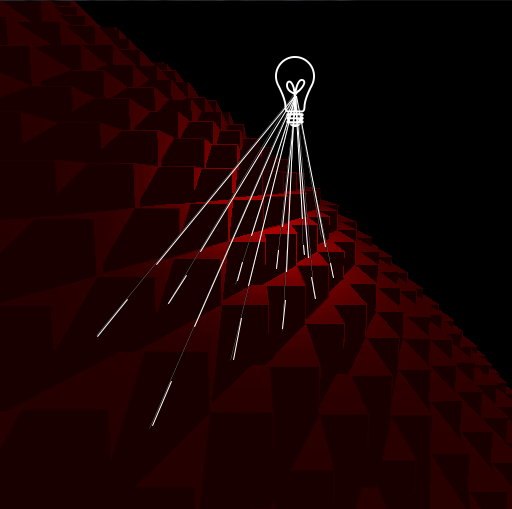
\includegraphics[width=6in]{ray_path.png}}

	\caption{The path of a shadow ray from the surface. The ray does not make it to the light, as it intersects with other voxels first}
	\label{fig:shadow-problem-ray-path}
\end{figure}

\begin{figure}
	\centering
	\subfloat[]{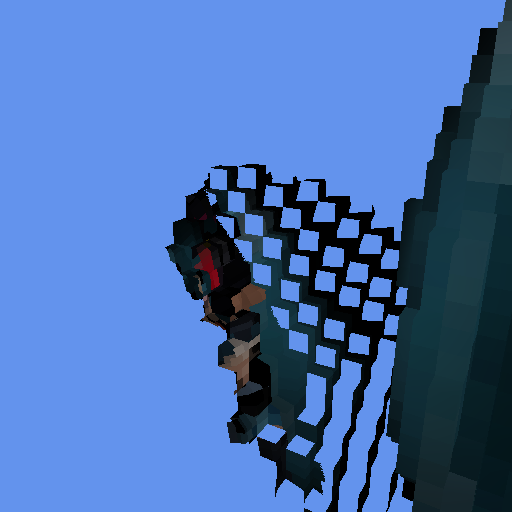
\includegraphics[width=4in]{voxel_problem_reflection.PNG}}

	\caption{The problem also occurs with reflection}
	\label{fig:shadow-problem-reflection}
\end{figure}

One possible solution to this problem is to increase the data resolution. As data resolution increases, the problem lessens. The problem with this solution is that it's hard to predict, in a general way, what resolution the data will need to be stored at in order to prevent these types of artifacts in any given situation. Even lessening the effect in this way is extremely memory inefficient.

There are two main alternatives to this solution. Since the problem only occurs for surface voxels, one possible solution is to make the ray casting algorithm aware of surface normals in order to perform a sort of back-face culling. The results of this are shown in figure \ref{fig:fixed-reflection}. The major disadvantage of doing this is that it adds a number of expensive calculations to the inner loop of the ray cast, greatly reducing the overall performance of the renderer. On top of this, it would be more desirable to extend such a solution to one that does not involve considering surfaces, in order to stay in line with our volumetric rendering goals.

\begin{figure}
	\centering
	\subfloat[]{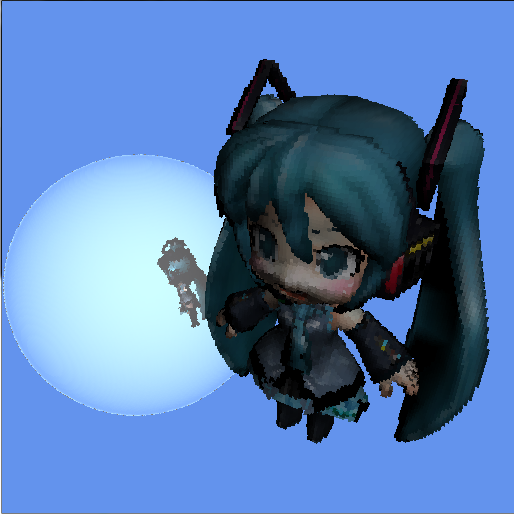
\includegraphics[width=4in]{fixed_reflection.PNG}}

	\caption{Making the ray casting algorithm aware of the normals of surfaces can solve the problem, but has disadvantages}
	\label{fig:fixed-reflection}
\end{figure}

A more generic version of this solution would use non-cubical voxels in order to improve the approximation a voxel can make of a surface. \citeauthor{laine10efficientsvos}'s contours technique, which can efficiently consider non-cubic voxels using a pair of parallel planes to bound a volume inside the voxel, does this. We believe that this technique would also solve our problems in this area, as well as greatly lessening the memory usage of our structure as discussed in section \ref{sec:memusage}.
\chapter{Future Work}
\label{future_work}
\section{Conclusion}

% Show bibliography
\nocite{*}
\printbibliography

% Use letters for appendices
\renewcommand\thesection{Appendix \Alph{section}}
\renewcommand\thesubsection{\arabic{subsection}}

% Include appendicies
\addcontentsline{toc}{chapter}{Appendices}
\appendix
\section{Source code}

\subsection{Hello, world!}

\lstset{language=C++}
\begin{lstlisting}
int main(int argc, char** argv)
{
	printf("Hello, world!");
}
\end{lstlisting}

\end{document}

